\documentclass[]{article}
\usepackage[margin=1in]{geometry}
\usepackage{physics}
\usepackage{color,soul}
\usepackage{comment}
\usepackage[toc,page]{appendix}
\usepackage[nottoc]{tocbibind}
\usepackage[english]{isodate}
\usepackage{authblk}

<<<<<<< .merge_file_cKYZ1o
\usepackage{graphicx}
\graphicspath{{Images/}}


\title{Vibronic effects on incoherent excitation in molecular systems}
=======

\title{Incoherently excited monomers at strong phonon coupling}

>>>>>>> .merge_file_pvGeVo
\author[1]{H. Maguire}
\affil[1]{Photon Science Institute and School of Physics and Astronomy, The University of Manchester, Oxford Road,
	Manchester M13 9PL, United Kingdom}

\begin{document}
\tableofcontents
\section*{Preface}
<<<<<<< .merge_file_cKYZ1o
Electron-phonon coupling theory from the book chapters.
\maketitle
\begin{abstract}
The conversion of incoherent electromagnetic energy into useful work in photovoltaic cells can be viewed in a heat-engine picture, with electrons being excited to the conduction band by hot, solar photons and electron-hole recombination occurring radiatively and non-radiatively due to cold phonon baths and the ambient vacuum. In this simplified classical scenario, all recombination effects (apart from those occurring across the target load) detract from the photocell efficiency, since they result in an unavoidable dissipation of energy.

Attempting to generate photocurrent via the same method in systems of just a few molecules works in much the same way, however now the likelihood of quantum coherence being present in the dynamics increases somewhat (due to the ) In the quantum picture, the presence of electronic coherence means that , some of these noise processes are thought to bring abo
In these notes we aim to investigate the interplay between vibrational and electronic degrees of freedom in the context of incoherently excited molecules. In essence it is a problem of introducing multiple baths at different orders of perturbation. In the limit of strong and intermediate exciton-phonon coupling, the interaction between an incoherent optical field and the effective system eigenstructure gives rise to a rich augmentation of the dynamics and steady states. Aim to answer the question, "what effect does having a well defined vibronic manifold have on the discrepancies between secular and non-secular optical master equations?" How does the reaction coordinate picture relate to the theory of delocalised (phonon?) vs localised vibrations (from the electron-phonon chapter). 

Recently, many models for novel nanoscopic photocells have been proposed based on architectures similar to those found in photosynthetic organisms. These natural light harvesting systems are considered to be highly efficient machines and more recently have exhibited quantum coherence on similar timescales to the underlying charge dynamics. Although its precise origin is unknown, theoretical work has considered whether this coherence may contribute to the high efficiency. Some suggest that the coherent signatures observed in time-resolved spectroscopy may be due to strong interactions between vibrational and electronic degrees of freedom within the underlying molecular system. 
Previous work has assumed weakly-coupled molecular vibrations and introduced decoherence via simple rate equations. In this work, we show that strongly-coupled vibrations change the way that the molecules interact with the incident solar photons and hence fundamentally alter the charge dynamics in molecular systems. Even for single molecules, this strong vibronic coupling can lead to rich non-equilibrium effects and qualitatively different steady states to the weak-coupling theory. In principle, this will affect the operational efficiency of photocells. \\

\end{abstract}
 
\section{TODO:}
\begin{itemize}
	\item Put the dynamics and manifold plots side-by-side
	\item Make smoother steady state plots
	\item Shift the sharp peak up in energy and investigate dynamics when a localised vibration is near resonance with a transition
\end{itemize}
\section{Introduction}
\textbf{Questions we need to answer for introduction:}
=======

\maketitle
\begin{abstract}
Here we study a single electronic transition in a molecule, which is interacting strongly with broad low-frequency phonons. Specifically, we aim to investigate how incoherent excitation from a weakly-coupled thermal radiation field affects these systems. The Reaction Coordinate (RC) mapping is applied to the electron-phonon coupling in order to extend the validity of a Born-Markov master equation by effectively redrawing the boundary between system and bath to include a collective phonon degree-of-freedom within the system. The RC method without external driving is compared to an exact solution. Eigenstates of the Hamiltonian in the RC frame represent mixed electron-phonon excited states - each state interacting with the ambient electromagnetic field differently. The various approximations that can be made on the electromagnetic system-field interaction can be broken by different phonon-coupling regimes. At strong system-environment coupling and high thermal field temperature, we see that the secular approximation breaks down in the quantum optical master equation, leading to different coherence dynamics.
\end{abstract}
 
\section{Plan:}
\begin{enumerate}
	\item Overview of the field and what is the motivation for studying this.
	\item Quick introduction to electron-vibrational interactions and molecular physics.
	\item Exact solution of the independent boson model.
	\item Reaction coordinate things - comparison to exact solution and weak coupling. Phonon population wrt. $\Omega_{RC}$ - meaning.
	\item Electromagnetic field things. Super-ohmic spectral density?
	\item Vibronic physics. In this chapter I will write about all of the current checks I have been doing to understand the physics. Discuss what happens to manifolds when splitting becomes small, which states are populated for realistic temperatures. Analysis of dynamics in different regimes.
	\item Coherence times wrt splitting, RC frequency and phonon coupling.
	\item Emission Spectra - what does this say about the nature of electron-phonon interaction?
\end{enumerate}
\subsection{Questions}
>>>>>>> .merge_file_pvGeVo
\begin{itemize}
	\item How does bare coupling strength relate to Huang-Rhys Parameter
	\item Where does it say that exciton-phonon/vibration interactions are strong in biomolecular light-harvesting systems?
	\item Is it the low-frequency delocalised continuum of phonon modes that are strongly coupled? Or specific resonant vibrational modes?
	\item What motivates the use of the reaction coordinate method? What does it allow? What are the restrictions?
	\item Potential nanosystems which harvest or manipulate light are likely to be fabricated in the solid state, where low-frequency phonon modes are likely to interact strongly with electronic degrees of freedom. Give a few examples of potential architectures.
	\item The size of natural light harvesting systems means that the peak solar frequencies are likely to have wavelengths that span many molecular sites. This leads to various collective excitation and emission effects. In the strong vibrational regime this leads to rich dynamics and steady states which are likely to affect the operational efficiency of a machine.
	\item Aim to answer the question, "what effect does having a well defined vibronic manifold have on the discrepancies between secular and non-secular optical master equations?" 
	\item How does the reaction coordinate picture relate to the theory of delocalised (phonon?) vs localised vibrations (from the electron-phonon chapter). 
\end{itemize}
In these notes, the interplay between vibrational and electronic degrees of freedom are investigated in the context of incoherently excited molecules. In essence it is a problem of introducing multiple baths at different orders of perturbation. In the limit of strong and intermediate exciton-phonon coupling, the interaction between an incoherent optical field and the effective system eigenstructure gives rise to a rich augmentation of the dynamics and steady states which can be explored with the Reaction Coordinate technique.

<<<<<<< .merge_file_cKYZ1o
The references \cite{Creatore2013}\cite{Dorfman}[Amir's published paper] discuss proposals for nanoscopic photocells based on recent analyses of biological photosynthetic architectures. Natural light-harvesting systems are made up of many pigment molecules, which can have a nearest-neighbour spacing of less than a nanometer\cite{Adolphs2006}(check reference), leading to pigment-pigment couplings strong enough to cause excitations to delocalise. In this case the electronic excitations of the system are known as excitons, which are bound electron-hole pairs. The dynamics of the excited states are subject to many disorder processes, due to the conformational and vibrational motion of the protein scaffolds in which the pigments are embedded, as well as the localised intra-molecular vibrational modes of the pigments themselves\cite{}. The conformational motion is essentially static compared to all other system and interaction timescales and is observed as inhomogeneous broadening of the various spectra. The low-frequency vibrational modes, or phonons, can be delocalised over many pigment sites and along with the localised vibrations lead to many interesting observable effects.

Excitation of a electronic molecular transition leads to a reconfiguration of the equilibrium position of the nucleus. WE assume that the nuclear motion is far slower than that of the electron, so this electronic excitation amounts to a vertical transition to a higher lying potential well. In a typical diagram, nuclear displacement would be along the x-axis, so the upper potential well will be shifted to the right by some amount - related to vibronic coupling strength. Vibrational states in the upper potential well are occupied according to the vibronic transitional moment, or Franck-Condon overlap factors. Generally the nuclear configuration will be compressed in the excited electronic state, so molecule will occupy many vibrational modes which will in turn dissipate energy, causing the surrounding environment to heat up and the population to move to the vibrational ground state.The higher lying vibrational states then relax back to the potential minimum (assuming low-temperature) of the excited state on a fast timescale. This energy, dissipated to the vibrational environment, is called the reorganisation energy.
\begin{itemize}
	\item Homogeneous broadening of the emission and absorption spectra. Homogeneous due to the fact that the noise processes are resolved over experimental timescales?
	\item A renormalisation of system transition energies.
=======
Several recent papers have discussed proposals for nanoscopic photocells based on recent analyses of biological photosynthetic architectures\cite{Dorfman}\cite{Creatore2013}\cite{Killoran2015}\cite{Fruchtman2016}. Natural light-harvesting systems are made up of many pigment molecules, which can have a nearest-neighbour spacing of less than a nanometer\cite{Adolphs2006}, leading to pigment-pigment couplings strong enough to cause superpositions of different excited pigment states. In this case the electronic excitations are excitonic in nature - bound electron-hole pairs . The dynamics of the excited states are subject to many disorder processes, due to the conformational and low-frequency vibrational motion of the protein scaffolds in which the pigments are embedded, as well as the localised intra-molecular vibrational modes of the pigments themselves. The conformational motion is essentially static compared to all other system and interaction timescales and is observed as inhomogeneous broadening of the various spectra. The low-frequency vibrational modes, or phonons, can be delocalised over many pigment sites and along with the localised, inter-molecular vibrations lead to many interesting observable effects:
\begin{itemize}
	\item Homogeneous broadening of the emission and absorption spectra.
	\item Dissipation of electronic energy into the vibrational environment as heat - known as the reorganisation energy.
	\item Dephasing of the excitonic wavefunction, leading to decoherence.
	\item A renormalisation of system transition energies and a polaron shifted excited state manifold.
>>>>>>> .merge_file_pvGeVo
\end{itemize}
In these systems, it is thought that the strength of exciton-vibration interactions is on the same order as the excitonic energies and intermolecular couplings, which means that a perturbative treatment of this interaction may not be valid. We therefore use the Reaction Coordinate method, which allows for strong coupling to low-frequency environment modes and a degree of non-Markovianity. 
\\
Light-harvesting systems also operate under incoherent driving by the incident electromagnetic field from the Sun. In organic systems, the average photon number at any time is usually very low, often motivating the study of dynamics in only the single-excitation subspace. This also means that often the process of absorption is ignored and the system is initially considered to be in an electronically excited state - with electromagnetic relaxation treated phenomenologically. Preparing the system in this way is also justified by the process of absorption occurring at a far shorter time-scale ($\sim fs$) than other molecular dynamics, such as fluorescence ($\sim ns$) and vibrational relaxation ($\sim ps$). 

We are interested in how vibronic systems continually interact with the electromagnetic field and so derive a Born-Markov master in the Reaction-Coordinate picture. We treat this master equation at various levels of approximation in order to understand which processes are likely to contribute in real systems.

A number of different approaches are
\begin{enumerate}
	\item Studying how strong-coupling leads to a breakdown of approximations of optical master equations. Spectral signatures.
	\item Choosing an appropriate regime and looking at how vibronic coupling affects dynamics and steady-states. Temperature dependence and 
\end{enumerate}

\subsection{Electron-vibration interaction}

Vibronic transitions are simultaneous electronic and vibrational transitions, most commonly found in molecular and quantum dot systems. Molecular vibrations can be thought of as the oscillations around the equilibrium distribution of an electron and the nucleus. When an electron is excited in a molecule it moves out further from the nucleus so it has a different distribution thus exerting a different force. The nuclei respond and the whole system changes its vibrational character, often breaking into more vigorous motion. In the Franck-Condon picture, it is assumed that nuclei take far longer to move than electrons so electronic transitions are essentially \emph{instantaneous}. In a typical diagram, with equilibrium nuclear displacement along the x axis and energy along the y-axis, both the ground and excited electronic states represent large potential wells, with vibrations forming separate ladders of states within each of them. The upper state is normally displaced to the right, since the entire potential energy of the molecule and thus the displacement is increased.

Since the nuclei adjust much more slowly than the electrons, the transition to the upper state occurs vertically. The upper state is usually compressed out of equilibrium so will vibrate more vigorously, occupying higher lying vibrational states. Excitation energy is then dissipated on a fast timescale into the vibrational modes of the molecular environment causing the excitation to relax to the bottom of the upper potential well (assuming $KT\ll\hbar\epsilon$ where T is temperature and $\epsilon$ is the TlS splitting). WE should expect to see the expected displacement of the phonons (in the Reaction-Coordinate density matrix) move between the two potential wells over the excited state life-time.

<<<<<<< .merge_file_cKYZ1o
In the case where vibrations couple strongly to electronic transitions, it has been shown that 
 In these systems, it is thought that the strength of exciton-phonon interactions is on the same order as the excitonic energies and intermolecule couplings, which means that we cannot use a perturbative treatment of this interaction. We therefore use the Reaction Coordinate method, which allows for strong coupling to low-frequency environment modes and a degree of non-Markovianity. 
\\ 

%\\ \textbf{How I'm going to write this thing:}
%\begin{itemize}
%	\item Go through and loosely write out the algebra and a loose discussion.
%	\item Read Ahsan and Jake's notes and try to include the types of arguments that they make.
%	\item Flesh out the discussion.
%	\item Choose a consistent notation and vocabulary.
%\end{itemize}

Things I still want to cover:
\begin{description}
	\item[Light-Harvesting] - 
	\item[Exciton-phonon coupling] - How does bare coupling strength relate to that electron-phonon coupling number they use in the literature?
	\item[Strong-coupling] - 
	\item[Incoherent driving] - 
	\item[TYPICAL PARAMETERS] - I need to have a range of parameters which are typical for the types of systems I am interested in. System splitting, electron-phonon coupling strength, phonon frequencies, vibrational frequencies, phonon cutoff frequency. Let's assume that natural systems are the most efficient and use these values.
\end{description}
\section{Non-perturbative Electron-Phonon coupling}
\begin{itemize}
=======
\section{Non-perturbative Exciton-Phonon coupling}
\begin{itemize}
	\item As we have mentioned, strong-coupling to vibrations can occur in biomolecular and solid state systems.
	\item Reaction coordinate method shown to be effective in modelling the broad and sharply peaked lorentzian sprectral densities, strong-coupling and non-Markovianity.
>>>>>>> .merge_file_pvGeVo
	\item Discuss RC regime of applicability, it's physical interpretation and precisely how this applies to the biomolecular problem.
\end{itemize}

 Considering only the system and phonon bath initially we have $H = H_S + H_I^{ph}$
\begin{equation}
H = \epsilon \dyad{X} + \alpha_{ph}\dyad{X}\sum_{k}(C^{\dagger}_k+C_k) + \sum_{k}\omega_k C^{\dagger}_k C_k.
\end{equation}
We apply a normal mode transformation in order to exactly map the normal independent boson model to the collective coordinate model
\begin{equation}
H = \epsilon \dyad{X} + \eta a^{\dagger}a + \lambda\dyad{X}(a^{\dagger}+a) + \sum_{k}h_k(a^{\dagger}+a)(c^{\dagger}_k+c_k) + \sum_{k}\omega_k c^{\dagger}_k c_k,
\end{equation}
whereby we define an oscillator which  is a collective representation of the entire bath and incorporate it into our system Hamiltonian, coupled coherently to the system of interest. The oscillator is then coupled weakly to a phonon residual bath. In this setting, we enlarge our system Hamiltonian since we now explicitly keep track of the collective coordinate, but we do Performing this mapping has been shown to recover valid dynamics for similar problems, well into the strong-coupling regime.
We restrict ourselves to a Lorentzian spectral density, 
\begin{equation}
\label{eq:DrudeLorentzUnderdamped}
J_{SB}(\omega) = \frac{\alpha \Gamma \omega_0^2\omega}{(\omega_0^2-\omega^2)^2 + \Gamma^2\omega^2},
\end{equation}

which in the reaction-coordinate frame maps exactly to the ohmic spectral density $J_{RC} = \gamma \omega \exp(-\omega/\Lambda)$ in the limit that $\Lambda\to\infty$.
\begin{equation}
\label{eq:DrudeLorentzUnderdamped1}
J_{SB}  = \frac{4\gamma\Omega^2\lambda^2\omega}{(\Omega^2-\omega^2)^2 + (2\pi\Omega\gamma)^2\omega^2}.
\end{equation}
Thus $\Omega = \omega_0$, $\lambda=\sqrt{\pi \alpha \omega_0/2}$ and $\gamma=\Gamma/2\pi\omega_0$. This means that for the underdamped spectral density $\Gamma$, $\omega_0$ and $\alpha$ are all free parameters, as shown in [J chem phys] in the case of large $\omega_0$ this spectrum becomes the overdamped, Drude-Lorentz sprectral density where $\Gamma=\omega_0^2\omega_c^{-1}$.

\begin{figure}
<<<<<<< .merge_file_cKYZ1o
	%\includegraphics[width=0.5\textwidth]{"C:/Users/mbcxrhm2/Dropbox/PhD/1st year/TwoSpins/TwoSpinsNotes/Images/SpectralDensities".pdf}
	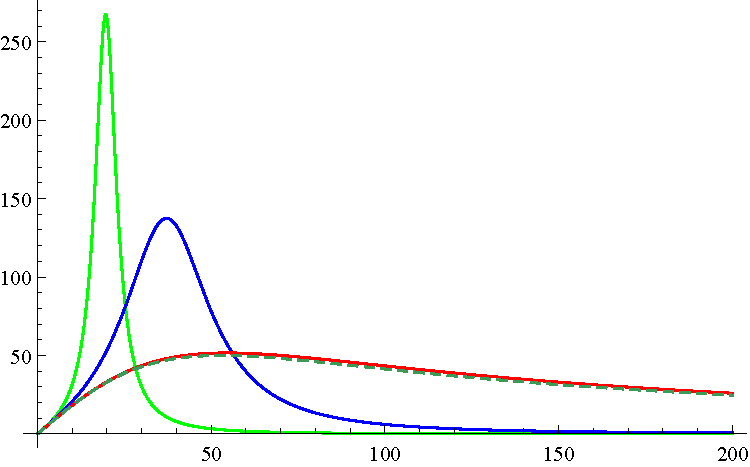
\includegraphics[width=0.5\textwidth]{Images/SDs/SpectralDensities.pdf}
=======
	\includegraphics[width=0.5\textwidth]{"/home/henry/Work/phd-work/vibronic-TLS/Notes/Images/SDs/SpectralDensities".pdf}
	%\includegraphics[width=0.5\textwidth]{"/home/henry/Dropbox/PhD/1st year/TwoSpins/TwoSpinsNotes/Images/SpectralDensities".pdf}
>>>>>>> .merge_file_pvGeVo
	\caption{Comparison of underdamped (solid lines) and overdamped (dashed line) spectral densities. Parameters are $\omega_c=53cm^{-1}$, $\alpha=100cm^{-1}$ and $\Gamma=\omega_0^2\omega_c^{-1}$.}
\end{figure}
\section{Exact Solution}
We start with the system and bath Hamiltonian
\begin{equation}
H = \epsilon\dyad{X} + \sum_{k}\omega_k b_k^{\dagger} b_k + \dyad{X}\sum_{k}g_k (b_k^{\dagger}+b_k)
\end{equation}
<<<<<<< HEAD
and perform a unitary, polaron transformation $H^{\prime} = e^{S}He^{-S}$ where $S= \dyad{X}\sum_{k}\frac{g_k}{\omega_k}(b_k^{\dagger}+b_k)$. This yields transformed system, bath and interaction Hamiltonians
=======
and perform a unitary, polaron transformation $H^{\prime} = e^{S}He^{-S}$ where $S= \dyad{X}\sum_{k}\frac{g_k}{\omega_k}(b_k^{\dagger}-b_k)$. This yields transformed system, bath and interaction Hamiltonians
>>>>>>> d91a73078751b16e271f9eb594f26a765226f8fc
\begin{align}
H_S^{\prime} &= \epsilon\dyad{X} \\
H_B^{\prime} &= \sum_{k}\omega_k b_k^{\dagger}b_k - \dyad{X}\sum_{k}g_k (b_k^{\dagger}+b_k) +\dyad{X}\sum_{k}\frac{g^2_k}{\omega_k} \\
H_I^{\prime} &= \dyad{X}\sum_{k}g_k (b_k^{\dagger}+b_k) - 2\dyad{X}\sum_{k}\frac{g^2_k}{\omega_k} \\
\end{align}
which together form the polaron-frame Hamiltonian
\begin{equation}
H^{\prime} = \epsilon\dyad{X} - \dyad{X}\sum_{k}\frac{g^2_k}{\omega_k} + \sum_{k}\omega_k b_k^{\dagger}b_k
\end{equation}
whereby the system and bath are now decoupled but the system energy has been renormalised due to the coupling - this is known as the polaron shift.

The time-evolution operator is thus
\begin{equation}
U^{\prime}(t) = e^{-i\epsilon\dyad{X}} e^{i\dyad{X}\sum_{k}\frac{g^2_k}{\omega_k}} e^{-i\sum_{k}\omega_k b_k^{\dagger}b_k}.
\end{equation}
We will now show that in the polaron frame the environmental modes undergo a shift dependent on whether the system is in the ground or excited state. We split up the full original  Hamiltonian
\begin{equation}
H_0 = \epsilon \dyad{X} + \sum \omega_k b_k^{\dagger}b_k \quad \textnormal{and} \quad H_I = \dyad{X}\sum g_k \dyad{X}
\end{equation}
in order to write 
\begin{align}
\tilde{U}(t) = e^{i H_0 t}U(t) &= e^{i H_0 t}e^{-S}U^{\prime}(t)e^{S} \\
&= e^{i H_0 t}e^{-S}e^{-i H_0 t}e^{i H_0 t}U^{\prime}(t)e^{S}
\end{align}
where we have made use of the identity operator for the final equality, from which we identify
\begin{equation}
e^{i H_0 t}e^{-S}e^{-i H_0 t} = \exp(-\dyad{X}\sum\frac{g_k}{\omega_k}(e^{i\omega_k t}b_k^{\dagger} - e^{-i\omega_k t}b_k))
\end{equation}
\begin{equation}
e^{i H_0 t}U^{\prime}(t) = e^{i\sum_{k}\frac{g^2_k}{\omega_k}\dyad{X}t}.
\end{equation}
By using the theorem for bringing together operator exponentials $e^{A+B} = e^{A}e^Be^{-\comm{A}{B}/2}$, after some algebra we reach
\begin{equation}
\label{eq:compactTimeEvOp}
\tilde{U}(t) = e^{-i\Phi(t)}e^{\dyad{X}\sum(\alpha_k(t)b_k^{\dagger}-\alpha_k^*(t)b_k)}
\end{equation}
where $\Phi(t) = \sum\frac{g^2_k}{\omega_k^2}\sin{\omega_k t}-\frac{g_k^2}{\omega_k}t$ and $\alpha_k=(1-e^{i\omega_k t})\frac{g_k}{\omega_k}$. By performing a series expansion of the second exponent in $\tilde{U}(t)$ we get
\begin{equation}
\tilde{U}(t) = e^{-i\Phi(t)}\left(\dyad{0} + \dyad{X}\prod_{k} D\left(\alpha_k(t)\right)\right) 
\end{equation}
where we have introduced the displacement operator $D(\alpha_k(t))=\exp(\alpha_k(t)b_k^{\dagger}-\alpha_k(t)b_k)$. We assume that system and bath are initially in a product state $\rho(0) = \rho_S(0)\otimes\rho_B$ and that the bath is in thermal equilibrium. Using
\begin{equation}
\tilde{rho}_{ij}(t) = \bra{i}\Tr_B\left[\tilde{U}(t)\rho(0)\tilde{U}^{\dagger}(t)\right]\ket{j}
\end{equation}
we find that the populations are left unchanged by the interaction
\begin{equation}
\tilde{\rho}_{00}(t) =\rho_{00}(0)\dyad{0} \quad \tilde{\rho}_{11}(t) =\rho_{11}(0)\dyad{X}
\end{equation}
whereas the coherences evolve according to
\begin{align}
\rho_{10}(t) &= \rho_{10}(0)\Tr_B\left(\prod_k D(\alpha_k(t)\rho_B)\right) = \rho_{10}(0)e^{\Gamma(t)} \\
\rho_{10}(t) &= \rho_{01}(0)\Tr_B\left(\rho_B\prod_kD^{\dagger}(\alpha_k(t))\right) = \rho_{01}(0)e^{\Gamma^*(t)}
\end{align}
where we have defined the decoherence function
\begin{equation}
\Gamma(t)=\ln(\Tr_B\left(\prod_k D(\alpha_k(t))\rho_B\right))=\sum_k\ln\left(\expval{D(\alpha_k(t))}_B\right).
\end{equation}
This allows us to identify the Wigner characteristic function for bath mode $k$, 
\begin{equation}
\expval{D(\alpha_k)}_B = \exp(-\frac{1}{2}\abs{\alpha_k}^2\expval{\{b_k, b_k^{\dagger} \}})
\end{equation}
so the decoherence function becomes
\begin{equation}
\Gamma(t)=\sum_k -\frac{1}{2}\abs{\alpha_k}^2\expval{\{b_k, b_k^{\dagger} \}} = -\sum_k (1-\cos(\omega_k t))\frac{\abs{g_k}^2}{\omega_k^2} \coth(\frac{\omega_k}{2k_BT})
\end{equation}
where the second equality comes from the definition of $\alpha_k(t)$ after equation \ref{eq:compactTimeEvOp} and a fair amount of algebra. Then defining the spectral density $J(\omega)=f(\omega)\abs{g(\omega)}^2$ where $f(\omega)$ is the density of phonon states, we get
\begin{equation}
\Gamma(t) = -\int_{0}^{\infty}d\omega \frac{J(\omega)}{\omega^2} \coth(\frac{\omega}{2k_BT})(1-\cos(\omega t))
\end{equation}
\subsection{The reaction coordinate master equation}
Defining $A= (a + a^{\dagger})$, we get the master equation
\begin{align}
	\begin{split}
		\label{eq:ReactionMasterExpansion4}
		\pdv{\rho(t)}{t} &= -i\left[H_0, \rho(t)\right]\\
		&-\int_{0}^{\infty}\int_{0}^{\infty}d\omega d\tau 
		\left[A,\left[\tilde{A}(-\tau),\rho(t) \right]\right] J_{RC}(\omega) \coth(\frac{\beta \omega}{2})\cos(\omega \tau)\\ 
		-& i\int_{0}^{\infty}\int_{0}^{\infty}d\omega d\tau\left[A ,\biggr\lbrace\left[\tilde{A}(-\tau),H_0\right],\rho(t) \biggr\rbrace \right] J_{RC}(\omega) \frac{\cos(\omega \tau)}{\omega}.
	\end{split}
\end{align}
At this point we can include the integrals over $\tau$ and $\omega$ in the definitions of two new operators
\begin{align}
	\label{eq:NewRCOperators}
	\chi &\equiv \int_{0}^{\infty}\int_{0}^{\infty}d\omega d\tau  J_{RC}(\omega) \coth(\frac{\beta \omega}{2})\cos(\omega \tau) \tilde{A}(-\tau)\\
	\Xi &\equiv \int_{0}^{\infty}\int_{0}^{\infty}d\omega d\tau  J_{RC}(\omega) \frac{\cos(\omega\tau)}{\omega} \left[H_0, \tilde{A}(-\tau)\right]
\end{align}
We then write the system operators in the basis of RC-TLS eigenstates $\ket{\phi_n}$ which gives
\begin{equation}
A = \sum_{ij}\bra{\phi_i}A\ket{\phi_j} \dyad{\phi_i}{\phi_j}
\end{equation}
where $H_0\ket{\phi_n} = \phi_n\ket{\phi_n}$. Transforming to the interaction picture with respect to $H_0$, the system operators become
\begin{equation}
\tilde{A}(t) = \sum_{ij}\bra{\phi_i}A\ket{\phi_j} e^{i(\phi_i-\phi_j)t}\dyad{\phi_i}{\phi_j}.
\end{equation}

Substituting this into (\ref{eq:NewRCOperators}) and integrating using 
\begin{equation}
	\label{eq:Sokhotski}
	\int_{0}^{\infty}f(\omega)d\omega\int_{0}^{\infty}d\tau e^{\pm i(\omega-\eta)\tau} = \pi\int_{0}^{\infty}f(\omega)\delta(\omega-\eta)d\omega \pm i \mathcal{P}\left[\int_{0}^{\infty}\frac{f(\omega)}{\omega-\eta}d\omega\right],
\end{equation}
yields
\begin{align}
	\label{eq:NewRCOperatorsDiscrete}
	\chi &\approx \sum_{ij}J_{RC}(\xi_{ij}) \coth(\frac{\beta \xi_{ij}}{2})\bra{\phi_i}A\ket{\phi_j}\dyad{\phi_i}{\phi_j}\\
	\Xi &\approx \sum_{ij}J_{RC}(\xi_{ij}) \bra{\phi_i}A\ket{\phi_j}\dyad{\phi_i}{\phi_j}
\end{align}
where $\xi_{ij} = (\phi_i-\phi_j)$ and the imaginary Lamb-shift terms have been neglected, justified in by benchmarking. These operators can be calculated by numerically diagonalising the TLS-RC system Hamiltonian $H_0$. This allows us to write the Reaction Coordinate master equation as
\begin{equation}
\pdv{\rho(t)}{t} = -i\left[H_0, \rho(t)\right] - \left[A, \left[\chi, \rho(t)\right]\right] + \left[A, \big\lbrace\Xi, \rho(t)\big\rbrace\right].
\end{equation}
\subsection{Weak Coupling Master Equation}
Deriving a Born-Markov master equation, converting back to Schr\"odinger picture and then spectrally decomposing the system operator in order to include time-dependence in terms of system eigenstates
$A(t)=\sum_{\zeta}A(\zeta)e^{-i\zeta t}$, yields
\begin{align}
\dot{\rho}_S(t) = -i[H_S, \rho_S(t)] -\frac{1}{2}\sum_{\zeta}&\gamma(\zeta)\big([A, A(\zeta)\rho_S(t)-\rho_S(t)A^{\dagger}(\zeta)]\\-&iS(\zeta)\big([A, A(\zeta)\rho_S(t)+\rho_S(t)A^{\dagger}(\zeta)]\big).
\end{align}
Full Hamiltonian of TLS plus phonon bath
\begin{equation}
H = \epsilon\dyad{1}{1} + \sum_{k}\omega_k a^{\dagger}_k a_k + \dyad{1}{1}\sum_{k} (a_k +a^{\dagger}_k) 
\end{equation}
Thus the interaction Hamiltonian in the interaction picture is
\begin{equation}
\tilde{H}_I(t) = \dyad{1}{1}\sum_{k} (a_ke^{-i\omega_k} +a^{\dagger}_ke^{i\omega_k}) 
\end{equation}
where in the interaction picture $O(t)=e^{i\omega_k}Oe^{-i\omega_k}$. Therefore the system operator $A = \dyad{1}$ is 
\begin{equation}
\quad \tilde{A}(t) = \dyad{1} = A.
\end{equation}

Plugging all this into the ME above we have
\begin{align}
\dot{\rho}_S(t) = -i[H_S, \rho_S(t)] -\frac{1}{2}&\gamma(0)\bigg(\big\{\dyad{1},\rho_S(t)\big\} - 2\dyad{1}\rho_S(t)\dyad{1}\bigg)\\-&iS(0)\big[\dyad{1},\rho_S(t)\big].
\end{align}
Where $\gamma(\omega)=2\Re{K(\omega)}$ and $S(\omega)=\Im{K(\omega)}$ with
\begin{equation}
K(\omega) = \int_{0}^{\infty}d\tau C(\tau)e^{i\omega\tau}.
\end{equation}
Calculating the above and evaluating the Fourier transform wrt zero gives $\gamma(0)=\lim\limits_{x\to0}\frac{\pi}{2}J(x)\coth(\beta x/2)$ and $S(0)=\int_{0}^{\infty}\frac{J(\omega)}{\omega}$.
In the case of electron-phonon interactions within molecular systems, it is reasonable to assume a Lorentzian spectral density
\begin{equation}
J(\omega) = \alpha \frac{\Gamma \omega_0^2 \omega}{(\omega_0^2 - \omega^2)^2 + \Gamma^2\omega^2}
\end{equation}
where $\alpha$, $\omega_0$ and $\Gamma$ describe the height, position and width of the Lorentzian. Defining a cutoff frequency $\omega_c$ and then defining $\Gamma = \omega_0^2/\omega_c$ where $\omega_0>>\omega_c$ gives a Drude-Lorentz or overdamped type spectral density.

\subsection{Dynamics}
\begin{figure}[t]
	\centering
	\begin{minipage}[b]{0.325\textwidth}
		\includegraphics[width=\textwidth]{"Images/PhononOnly/Phonons\string_only\string_weak".pdf}
		\caption{TLS Site Coherence: Weak-Coupling Regime. The weak coupling theory matches the exact solution.}
		\label{fig:PhononOnlyWeak}
	\end{minipage}
	\begin{minipage}[b]{0.325\textwidth}
		\includegraphics[width=\textwidth]{"Images/PhononOnly/Phonons\string_only\string_intermediate".pdf}
		\caption{TLS Site Coherence: intermediate-Coupling Regime. Broad, overdamped Lorenztian Phonon bath. $\omega_{c}=53cm^{-1}$ $\pi\alpha=1000cm^{-1}$}
		\label{fig:PhononOnlyIntermediate}
	\end{minipage}
	\begin{minipage}[b]{0.325\textwidth}
		\includegraphics[width=\textwidth]{"Images/PhononOnly/Phonons\string_only\string_strong".pdf}
		\caption{TLS Site Coherence: Strong-Coupling Regime. Broad, overdamped Lorenztian Phonon bath.}
		\label{fig:PhononOnlyStrong}
	\end{minipage}
\end{figure}

\begin{figure}
	\centering
	\begin{minipage}[b]{0.45\textwidth}
		\includegraphics[width=\textwidth]{"Images/PhononOnly/Phonons\string_only\string_strong\string_resonantOD\string_G10".pdf}
		\caption{TLS Site Coherence: Strong-Coupling Regime. Sharply peaked underdamped Lorenztian Vibrational mode. $\omega_0=\epsilon$, $\Gamma=100cm^{-1}$, $\alpha=1000cm^{-1}$}
		\label{fig:PhononOnlyStrongOD}
	\end{minipage}
	\begin{minipage}[b]{0.45\textwidth}
		\includegraphics[width=\textwidth]{"Images/FrequencyAnalysis/noPhononFreqSpectra".png}\caption{Fourier transform of figure \ref{fig:PhononOnlyStrongOD}.}
		\label{fig:PhononOnlySpectra}
	\end{minipage}
\end{figure}
In figure \ref{fig:PhononOnlyWeak} we can see that the weak coupling theory is only valid in very weak coupling regimes. The Reaction Coordinate model seems to agree well with the exact calculation well into the strong-coupling regime, for broad, overdamped Spectral densities. However, as the phonon bath spectral density gets narrower the RC method breaks down as seen in \ref{fig:PhononOnlyStrongOD}.
\section{Vibronic dissipation due to an electromagnetic bath}
We now want to investigate the behaviour of the vibronic system when coupled to the ambient electromagnetic field, where the overall Hamiltonian is
\begin{equation}
H = H_S + H_I^{Vib} + H_B^{Vib} + H_I^{EM}+ H_B^{EM}.
\end{equation}

Firstly, we calculate the effect of the electromagnetic bath on vibronic excitations, where the electronic degree of freedom is a single excitation in a molecule and the vibrations are delocalised (over the solid state substrate or protein scaffold) leading to a broad overdamped Lorentzian profile. In the literature, \textit{vibronic} systems usually comprise of electronic and localised, intra-molecular vibrational modes (sharp) often taken to be a single oscillator mode. Since we use the RC mapping, where a single oscillator does strongly couple to the electronic transition we will also use the term \textit{vibronic} to describe the new diagonal system basis - even if the underlying spectrum is broad.

For a two-level system coupled to an electromagnetic bath there are a variety of gauges we can choose for the electromagnetic coupling. In \cite{Stokes2012}, the minimal coupling for
\begin{equation}
\label{eq:MinimalCouplingConst}
f_{k\lambda} = i e \left(\frac{\omega_0}{2\epsilon_0 L^3}\right)^{\frac{1}{2}} \vec{e}_{k \lambda}\cdot\vec{d} \left(\frac{\omega_0}{\omega_k}\right)^{\frac{1}{2}} 
\end{equation}
and the multipolar form
\begin{equation}
\label{eq:MultipolarCouplingConst}
g_{k\lambda} = i e \left(\frac{\omega_0}{2\epsilon_0 L^3}\right)^{\frac{1}{2}} \vec{e}_{k \lambda}\cdot\vec{d} \left(\frac{\omega_k}{\omega_0}\right)^{\frac{1}{2}} 
\end{equation}
are used. 
In the case of the minimal coupling, this leads to the spectral denisty
\begin{equation}
J(\omega) = \left(\frac{\pi e^2\omega_0^2 |d|^2}{2\epsilon_0(3\pi^3 c^3)}\right)\omega.
\end{equation}
For the two-level system the two different forms of coupling lead to the same spontaneous emission rates since the resultant spectral densities are evaluated at the same TLS splitting frequency
\begin{equation}
\label{eq:TLS_decay}
\Gamma = 2\pi J(\omega_0) = \pi\left(\frac{\pi e^2\omega_0^2 |d|^2}{2\epsilon_0(3\pi^3 c^3)}\right)\omega_0,
\end{equation}
which means the constants can be expressed
\begin{equation}
\frac{\pi}{2} \frac{e^2\abs{\vec{d}}^2}{3\epsilon_0\pi^3c^3} = \frac{\Gamma}{2\pi\omega_0}.
\end{equation}
For a real molecule, it may not be easy to measure the dipole strength of a transition, but it might be easy to gain access to the (zero-phonon) excited state lifetime ($T_1 \approx 100ps - 1ns$) which gives a value for spontaneous emission rate ($\Gamma\approx 10^9-10^{10}s^{-1}$). We could then express the spectral density in terms of this
\begin{equation}
\label{eq:MinimalSpectral}
J_{mc}(\omega) = \frac{\Gamma\omega}{2\pi\omega_0}.
\end{equation}
For the multipolar gauge we have
\begin{equation}
\label{eq:MultipolarSpectral}
J_{mp}(\omega) = \frac{\Gamma\omega^3}{2\pi\omega_0^3}
\end{equation}
from which it can be seen that $\Gamma_{TLS}=J_{mc}(\omega_0)=J_{mp}(\omega_0)$, i.e. that the system-bath coupling and decay rates are gauge-invariant when evaluated at the TLS frequency.

The many high-lying vibronic states on both the excited and ground manifold mean that even for a single electronic transition there are many vibronic transition frequencies and the transition rates between them are going to depend strongly on the overlap of the various vibrational wavefunctions. 

As we will see later, the vibronic transition rates for the process $\ket{\phi_q}\to\ket{\phi_p}$ due to electromagnetic field interaction, as described by a secular Born-Markov master equation (ignoring Lamb-shifts) is given by
\begin{equation}
\Gamma_{pq} = \pi J(\omega_{pq}) A_{p,q}^{*}A_{p,q}
\end{equation}
where $A_{p,q}=\bra{\phi_p}\sigma\otimes I_{RC}\ket{\phi_q}$ and the vibronic system eigenstates are defined $H_S\ket{\phi_i}= \omega_i\ket{\phi_i}$.

The question is: \textit{how does each vibronic state couple to the electromagnetic field?} Now, the complete answer to this question may require detailed knowledge about the various vibronic dipole moments and for this to be input into something of the form of equation \ref{eq:MinimalCouplingConst}. This information could possibly be obtained from ab initio calculations such as DFT(?), but it is not necessary for our applications.

In our model the underlying way that the vibronic system couples to the field is via the electronic transition. This means that we do not expect the form of the coupling to the system-bath coupling to change substantially once we include the vibrational mode. Instead it is likely that the frequency dependence of the coupling as seen in the spectral density \ref{eq:MinimalSpectral} dominates the physics, rather than the coefficients. If this is accurate then we can incorporate much of the physics by simply using evaluating the TLS-optical field spectral density at the various vibronic frequencies. One remaining problem is that now the rates of the form \ref{eq:TLS_decay} are no longer gauge-invariant. This means that we need to check whether our choice of gauge qualitatively affects the physics.

\begin{figure}[t]
	\centering
	%\includegraphics[width=0.8\textwidth]{"/home/henry/Work/phd-work/vibronic-TLS/Notes/Images/Diagrams/rates_N6_a_ph400".pdf}
	\includegraphics[width=0.8\textwidth]{"/home/henry/Work/phd-work/vibronic-TLS/Notes/Images/Diagrams/rates_N6_a_ph400".pdf}
	\caption{Spontaneous decay rates for the various non-secular master equation terms as given by the real, temperature independent terms in \ref{eq:VibronicNonSecular1}, vs the transition frequency differences. The blue vertical lines are factors of the polaron-shifted TLS frequency. Yellow points are those which are forbidden by having zero transition dipole moment. The blue points are the terms left over after a strict, secular approximation has been made. $\alpha_{ph}=400 cm^{-1}$, $T_{EM} =6000$, $\hbar\omega_0 = 300cm^{-1}$}
	\label{fig:DecayRates_FrequencyDiffs}
\end{figure}

In figure \ref{fig:DecayRates_FrequencyDiffs} we see that for a TLS the various transition frequency differences form five bands, centered around $\pm2\epsilon$, $\pm\epsilon$ and zero.
\subsection{Non-Rotating Wave Approximation}
\label{ssec:nrwa}
Here we derive a Born-Markov master equation (Redfield equation) for the light-matter coupling without imposing the rotating wave approximation. The idea is that since the coupled system-vibrational Hamiltonian has potentially degenerate eigenfrequencies spanning many orders of magnitude there may exist some combination of transitions which become non-negligibly coupled by the shared optical field which are \textit{counter-rotating} but slowly. The Hamiltonian for the dissipative vibronic system is $H = H_S + H_B^{Vib} + H_I^{Vib} + H_B^{EM} + H_I^{EM}$
\begin{align}
\label{eq:H_nrwa}
	\begin{split}
		H_S &= \epsilon \sigma^{\dagger}\sigma\otimes I_{RC} + \eta\sigma^{\dagger}\sigma(c + c^{\dagger}) + \Omega ( I_{TLS}\otimes c^{\dagger}c) \\
		H_B^{EM} &= \sum_{j}\omega_j b^{\dagger}_j b_j \quad \quad H_I^{EM} = \sum_{j}(\sigma+\sigma^{\dagger})(g_j^*b^{\dagger}_j+ g_j b_j).
	\end{split}
\end{align}
From this we derive a master equation in the Born-Markov approximation for an weakly-coupled system-bath interaction $H_I(t)$ of arbitrary form
\begin{equation}
\pdv{\rho(t)}{t} = -i[H_S, \rho_S(t)] -\int_{0}^{\infty}d\tau\tr\left(\left[H_I, H_I(-\tau)\rho(t)\right] - \left[H_I, \rho(t)H_I(-\tau)\right]\right)
\end{equation}
where we are integrating over all time-differences $\tau$ by assuming a separation of time-scales between the system dynamics and the bath correlations, we have also assumed that the full density operator is separable $\tilde{\rho}(t) = \tilde{\rho_S}(t)\otimes\tilde{\rho_B}(t)$ for all times $t$. Since we are concerned with the interaction between the system of interest and the electromagnetic field, we transform $H_I^{EM}$ to the interaction picture with respect to the $H_S + H_B$ which accounts for the full vibronic eigenstructure. Here we take advantage of the fact that the interaction Hamiltonian is of the form $H_I^{EM}=AB$ where $A \equiv \sigma + \sigma^{\dagger}$ and $B\equiv \sum_{j}(g_j^*b^{\dagger}_j+ g_j b_j)$ and the fact that $H_B$ and $H_S$ commute.
Eventually we get
\begin{equation}
\label{nRWA_master}
\pdv{\rho(t)}{t} = -i[H_S, \rho_S(t)] - \left[\sigma_x, Z\rho_S(t)\right] - \left[\rho_S(t) Z^{\dagger}, \sigma_x\right]
\end{equation}
where
\begin{equation}
Z = \int_{0}^{\infty}d\tau C(\tau)A(-\tau)
\end{equation}
and
\begin{equation}
C(\tau) = \int_{0}^{\infty}d\omega J(\omega)\left(\coth(\frac{\beta \omega}{2}) \cos\omega\tau - i\sin\omega\tau\right).
\end{equation}
We can calculate the operator $Z$ numerically by expressing the system operator in terms of eigenstates of $H_S$ such that $H_S\ket{\varphi_m}=\varphi_m\ket{\varphi_m}$ so we have
\begin{equation}
\label{eq:Adecomposition}
A(t) = \sum_{m,n} A_{m,n} e^{i\xi_{mn}t}\dyad{\varphi_m}{\varphi_n}.
\end{equation}
In reality, this means we will have to truncate the Hilbert space of the RC. Bringing this all together yields
\begin{equation}
Z = \sum_{m,n} A_{m,n} \int_{0}^{\infty}d\tau \int_{0}^{\infty}d\omega J(\omega)\left(\coth(\frac{\beta \omega}{2}) \cos\omega\tau - i\sin\omega\tau\right)e^{-i\xi_{mn}t}\dyad{\varphi_m}{\varphi_n}
\end{equation}
which can be rewritten as
\begin{equation}
Z = \sum_{m,n} A_{m,n} \Gamma(\xi_{mn}) \dyad{\varphi_m}{\varphi_n}
\end{equation}
where the temperature-dependent rates are defined
\begin{equation}
\Gamma(\xi_{mn}) = \int_{0}^{\infty}d\tau \int_{0}^{\infty}d\omega \left(f_1(\omega)e^{i(\omega-\xi_{mn})\tau} + f_2(\omega)e^{-i(\omega+\xi_{mn})\tau}\right)
\end{equation}
along with the functions
\begin{equation}
f_1(\omega) = \frac{1}{2}J(\omega)(\coth(\beta \omega/2)-1) \quad \textnormal{and} \quad f_2(\omega)= \frac{1}{2}J(\omega)(\coth(\beta \omega/2)+1).
\end{equation}
The rates can be evaluated using \ref{eq:Sokhotski}
\begin{equation}
\Gamma(\xi_{mn}) =
\begin{cases}
\pi f_1(\xi_{mn}) + i\mathcal{P}\left[\int_{0}^{\infty}\left(\frac{f_1(\omega)}{\omega-\xi_{mn}} - \frac{f_2(\omega)}{\omega+\xi_{mn}}\right)d\omega\right] & \text{if } \xi_{mn}>0,\\ 
\frac{\pi}{2}\lim\limits_{x\to 0}\left(J(x)\coth(\frac{\beta x}{2})\right) - i\mathcal{P}\left[\int_{0}^{\infty}\frac{J(\omega)}{\omega}d\omega\right] & \text{if } \xi_{mn}=0,\\ 
\pi f_2(\abs{\xi_{mn}}) + i\mathcal{P}\left[\int_{0}^{\infty}\left(\frac{f_1(\omega)}{\omega+\abs{\xi_{mn}}} - \frac{f_2(\omega)}{\omega-\abs{\xi_{mn}}}\right)d\omega\right]  & \text{if } \xi_{mn}<0.
\end{cases}
\end{equation}
\begin{itemize}
	\item Limiting case: check for a TLS (no vibronic levels) what the master equation terms reduce to. Is there a way to make these terms have negligible effect, as in Ahsan's notes where $\alpha\ll \epsilon$. What would this mean for the vibronic system and which parameter regimes might satisfy this?
	\item What happens if you make the secular approximation? This is not possible for this master equation because I never looked at things in the interaction picture. Would we be interested in studying this?
\end{itemize}
\subsection{Vibronic non-secular theory}
\label{ssec:nsec}
Starting from \ref{eq:H_nrwa} we make a Rotating-Wave-Approximation (RWA) by discarding the counter rotating terms in the $H^{EM}_I$, yielding
\begin{align}
	\begin{split}
		H_S &= \epsilon \sigma^{\dagger}\sigma\otimes I_{RC} + \eta\sigma^{\dagger}\sigma(c + c^{\dagger}) + \Omega ( I_{TLS}\otimes c^{\dagger}c) \\
		H_B^{EM} &= \sum_{j}\omega_j b^{\dagger}_j b_j \quad \quad H_I^{EM} = \sum_{j}g_j\sigma b^{\dagger}_j+ g_j^*\sigma^{\dagger} b_j 
	\end{split}
\end{align}
We transform the interaction Hamiltonian to the interaction picture by $H_I(t) = e^{i(H_S+H_B) t}H_I e^{-i (H_S+H_B)t}$ which gives the form of coupling
\begin{equation}
\label{eq:IDecomposition}
H_I(t) = A(t) B^{\dagger}(t) + A^{\dagger}(t) B(t)  
\end{equation}
where $A(t) = e^{iH_S t}Ae^{-i H_S t}$, $A \equiv\sigma_\otimes I_{RC}$ and $B(t)= \sum_{j}g_ja_je^{-i\omega_j t}$. Since $H_S$ is a composite of two interacting subsystems, it is not straightforward to perform the matrix exponentiation and becomes useful to write down the system operator $A$ in terms of the eigenstates of $H_S$,
\begin{equation}
A \equiv \sigma\otimes I_{RC} = \sum_{m,n} \bra{\varphi_m}\sigma\otimes I_{RC}\ket{\varphi_n}\dyad{\varphi_m}{\varphi_n}
\end{equation}
such that $H_S\ket{\varphi_m}=\varphi_m\ket{\varphi_m}$. So we have the system operator as a superposition of various oscillatory components
\begin{equation}
\label{eq:Adecomposition}
A(t) = \sum_{m,n} A_{m,n} e^{i\xi_{mn}t}\dyad{\varphi_m}{\varphi_n}
\end{equation}
where $\xi_{mn} = \varphi_m - \varphi_n$ and $A_{m,n} = \bra{\varphi_m}A\ket{\varphi_n}$. When the interaction Hamiltonian can be written in this form, the second-order Born-Markov master equation can be expressed
\begin{align}
	\begin{split}
		\label{eq:BornMarkov}
		\pdv{\tilde{\rho}(t)}{t} = - \int_{0}^{\infty}& d\tau  \left[A(t), A^{\dagger}(t-\tau)\tilde{\rho}(t)\right] \expval{B^{\dagger}(\tau)B} + \left[A^{\dagger}(t),A(t-\tau)\tilde{\rho}(t)\right] \expval{B(\tau)B^{\dagger}} + h.c.,
	\end{split}
\end{align}
then substituting \ref{eq:Adecomposition} into this expression we get
\begin{align}
	\begin{split}
		\pdv{\tilde{\rho}(t)}{t} = - \sum_{l,m,p,q}\int_{0}^{\infty}& d\tau e^{-i(\xi_{lm}-\xi_{pq})t} e^{-i\xi_{pq}\tau} A_{l,m}A_{p,q}^{*}\big[\dyad{\varphi_l}{\varphi_m}, \dyad{\varphi_q}{\varphi_p}\tilde{\rho}(t)\big] \expval{B^{\dagger}(\tau)B} \\
		&+ e^{i(\xi_{lm}-\xi_{pq})t} e^{i\xi_{pq}\tau} A_{l,m}^{*}A_{p,q}\big[\dyad{\varphi_m}{\varphi_l}, \dyad{\varphi_p}{\varphi_q}\tilde{\rho}(t)\big] \expval{B(\tau)B^{\dagger}} + h.c.,
	\end{split}
\end{align}
where $A_{l,m}^*=\bra{\varphi_m}A^{\dagger}\ket{\varphi_l}$. The correlation functions can be written as
\begin{align}
	\begin{split}
		\expval{B^{\dagger}(\tau)B} = \tr\left(\sum_{k,k^{\prime}}e^{i\omega_k \tau}g_k^*g_{k^{\prime}} b_k^{\dagger}b_{k^{\prime}}\rho_E\right)\\
		\expval{B(\tau)B^{\dagger}}=\tr\left(\sum_{k,k^{\prime}}e^{-i\omega_k \tau}g_k^*g_{k^{\prime}} b_{k^{\prime}}b_k^{\dagger}\rho_E\right)
	\end{split}
\end{align}
which, after moving to the continuum limit in the number of environmental modes become;
\begin{align}
	\begin{split}
		\expval{B^{\dagger}(\tau)B} = \int_0^{\infty}d\omega e^{i\omega \tau}J(\omega)N(\omega)\\
		\expval{B(\tau)B^{\dagger}}=\int_0^{\infty}d\omega e^{-i\omega \tau}J(\omega)(N(\omega)+1)
	\end{split}
\end{align}
where $J(\omega)$ is the spectral density and $N(\omega)$ is the boson occupation number. From the delta function in \ref{eq:Sokhotski} real part of the integrals over time and frequency become decay rates evaluated at the differences in eigenfrequencies,
\begin{equation}
\gamma(\omega)=\pi J(\omega),
\end{equation}
the imaginary parts are the principal values of the integral which we denote $\Lambda_1$ and $\Lambda_2$. I'll leave these completely for now, but it's only important to know that the integrand of $\Lambda_2$ is $ \propto N(\omega)$ so disappear at zero temperature.
Moving back to the Schrodinger picture gives

\begin{align}
	\label{eq:VibronicNonSecular1}
	\begin{split}
		\pdv{\rho(t)}{t} = -i[H_S, \rho_S(t)] &- \sum_{l,m,p,q}  (N(\xi_{pq})\gamma(\xi_{pq})+i\Lambda_2(\xi_{pq})) A_{l,m}A_{p,q}^{*}\big[\dyad{\varphi_l}{\varphi_m}, \dyad{\varphi_q}{\varphi_p}\tilde{\rho}(t)\big] \\
		&+ (\gamma(\xi_{pq})(N(\xi_{pq})+1)-i(\Lambda_1(\xi_{pq})+\Lambda_2(\xi_{pq})))  A_{l,m}^{*}A_{p,q}\big[\dyad{\varphi_m}{\varphi_l}, \dyad{\varphi_p}{\varphi_q}\tilde{\rho}(t)\big]\\ &+ h.c.
	\end{split}
\end{align}
In order to justify the secular approximation in this case, we would have to show that an overdamped spectral density always gives negligible overlap coefficients $A_{l,m}A_{p,q}^{*}$ for nearly resonant transitions $\xi_{lm}\approx \xi_{pq}$.

There is no dipole-moment associated with transitions between vibrational states within the same electronic state manifold, therefore in the uncoupled basis
\begin{align}
	\begin{split}
		\bra{g,n}\sigma\ket{g,m} = \bra{e,n}\sigma\ket{e,m} = 0, \quad \textnormal{for any phonon modes } m,n.
	\end{split}
\end{align}
I predict that for an underdamped spectral density, the small value of $\Omega$ will mean that the two vibrational manifolds will be well separated so there will be no nearly degenerate states on separate manifolds, this should mean that any two transitions with a large overlap coefficient $A_{l,m}A_{p,q}^{*}$ will describe two far from resonance transitions and the secular approximation will be valid.

In reality, numerically calculating each of these terms is going to be expensive, since if the dimension of the Hilbert space of the RC is $D$ there could be $D^4$ terms in the master equation (although many terms will be zero). As we have seen in the RCME, it is possible to hide most of the non-secular information within some newly defined operators so that only a maximum $D^2$ terms need to be calculated. Taking the master equation \ref{eq:BornMarkov} and transforming back to the Schrodinger picture straight away we have
\begin{align}
	\begin{split}
		\label{eq:BornMarkovSchrod}
		\pdv{\rho(t)}{t} = -i[H_S, \rho(t)] - \int_{0}^{\infty}& d\tau  \left[A, A^{\dagger}(-\tau)\rho(t)\right] \expval{B^{\dagger}(\tau)B} + \left[A^{\dagger},A(-\tau)\rho(t)\right] \expval{B(\tau)B^{\dagger}} + h.c.
	\end{split}
\end{align}
We now substitute in \ref{eq:Adecomposition} and bring the integrals into new operators
\begin{align}
	\begin{split}
<<<<<<< .merge_file_cKYZ1o
		\pdv{\rho(t)}{t} = -i[H_S, \rho(t)] - \left[A, \chi_1 \rho(t)\right]  + \left[\rho(t)\chi_2,A\right] + h.c.
=======
		\pdv{\rho(t)}{t} = -i[H_S, \rho(t)] - \left[A, \chi_1\rho(t)\right]  + \left[\rho(t)\chi_2,A\right] + h.c.
>>>>>>> .merge_file_pvGeVo
	\end{split}
\end{align}
where 
\begin{align}
	\begin{split}
\chi_1 &= \sum_{m n}\int_{0}^{\infty}d\tau\int_{0}^{\infty}d\omega J(\omega)N(\omega)e^{i\omega\tau}A_{i,j}^* e^{i\xi_{mn}t}\dyad{\varphi_m}{\varphi_n} \\
\chi_2 &= \sum_{m n}\int_{0}^{\infty}d\tau\int_{0}^{\infty}d\omega J(\omega)(1+N(\omega))e^{-i\omega\tau}A_{i,j}^* e^{i\xi_{mn}t}\dyad{\varphi_m}{\varphi_n} 
	\end{split}
\end{align}

\begin{itemize}
	\item Discuss what all the terms and rates might mean.
	\item State the argument for a secular approximation and then explain why it is not generally valid in this case, with the figure of coefficients versus frequencies - it is the intermediate, nearly resonant region which is important, weight this by the decay rate so that it accounts for the fact that for the secular approximation to be valid the characteristic system frequency $\omega>\gamma$.
	\item In the case of the RC mapping, the effect is caused by a single phonon mode representing the entire bath. The problem is mapped exactly, does this mean these non-secular effects are real? If not, does this mean that dealing with multiple baths are a limitation of the RC model since the dynamics is mapped exactly only with the single bath? Surely if the Hamiltonians commute then it doesn't matter?
\end{itemize}


Here we derive the master equation which hides the non-secularity in those operators. We don't have as much physical insight when the problem is in this form, but it is far easier to numerically construct the Liouvillian.

\subsection{Vibronic Lindblad theory}
\label{ssec:sec}
Starting from \ref{eq:VibronicNonSecular1} we make the secular approximation anyway. This is to ensure that the map is completely positive and trace preserving, so always gives physical results for the two subsystem density matrices. This is a strong assumption and we are not expecting it to be correct, based on the evidence we have seen in the previous section, we just want to see the effect that the assumption has on the dynamics in various parameter regimes.

\begin{align}
	\label{eq:VibronicSecular1}
	\begin{split}
		\pdv{\rho(t)}{t} = -i[H_S, \rho_S(t)] &- \sum_{p,q}  (N(\xi_{pq})\gamma(\xi_{pq})+i\Lambda_2(\xi_{pq})) A_{p,q}A_{p,q}^{*}\big[\dyad{\varphi_p}{\varphi_q}, \dyad{\varphi_q}{\varphi_p}\tilde{\rho}(t)\big] \\
		&+ (\gamma(\xi_{pq})(N(\xi_{pq})+1)-i(\Lambda_1(\xi_{pq})+\Lambda_2(\xi_{pq})))  A_{p,q}^{*}A_{p,q}\big[\dyad{\varphi_q}{\varphi_p}, \dyad{\varphi_p}{\varphi_q}\tilde{\rho}(t)\big]\\ &+ h.c. \\
	\end{split}
\end{align}
\begin{align}
	\label{eq:VibronicSecular2}
	\begin{split}
		\pdv{\rho(t)}{t} = -i[H_S, \rho_S(t)] &- \sum_{p,q}  (N(\xi_{pq})\gamma(\xi_{pq})+i\Lambda_2(\xi_{pq})) A_{p,q}A_{p,q}^{*}\big(\dyad{\varphi_p}{\varphi_p}\tilde{\rho}(t) - \dyad{\varphi_q}{\varphi_p}\tilde{\rho}(t)\dyad{\varphi_p}{\varphi_q}\big) \\
		&+ (\gamma(\xi_{pq})(N(\xi_{pq})+1)-i(\Lambda_1(\xi_{pq})+\Lambda_2(\xi_{pq})))  A_{p,q}^{*}A_{p,q}\big(\dyad{\varphi_q}{\varphi_q}\tilde{\rho}(t) - \dyad{\varphi_p}{\varphi_q}\tilde{\rho}(t)\dyad{\varphi_q}{\varphi_p}\big)\\ &+ h.c. \\
	\end{split}
\end{align}
Due to the Hermitian conjugate terms, the imaginary parts either cancel out (the final term on each line) or become unitary Hamiltonian-like contributions
\begin{align}
	\label{eq:VibronicSecular2}
	\begin{split}
		\pdv{\rho(t)}{t} = -i[H_S^{\prime}, \rho_S(t)] &- \sum_{p,q}  N(\xi_{pq})\gamma(\xi_{pq}) A_{p,q}A_{p,q}^{*}\big(\{\dyad{\varphi_p}{\varphi_p}, \tilde{\rho}(t)\} - 2\dyad{\varphi_q}{\varphi_p}\tilde{\rho}(t)\dyad{\varphi_p}{\varphi_q}\big) \\
		&+ \gamma(\xi_{pq})(N(\xi_{pq})+1)  A_{p,q}^{*}A_{p,q}\big(\{\dyad{\varphi_q}{\varphi_q}, \tilde{\rho}(t)\} - 2\dyad{\varphi_p}{\varphi_q}\tilde{\rho}(t)\dyad{\varphi_q}{\varphi_p}\big) \\
	\end{split}
\end{align}
here we can see that making the secular approximation has resulted in a summation of many Lindblad operators, with collapse operators formed from the various vibronic eigenstates.

\subsection{Electronic Lindblad theory}
\label{ssec:electronic}
\begin{equation}
\lambda_{\pm} = \omega_2 + \frac{1}{2}(\epsilon \pm \eta)
\end{equation}
where $\omega_1 = \omega_2 +\epsilon$
\begin{equation}
\ket{\nu_\pm} = \frac{1}{\sqrt{2\eta}}\left(\sqrt{\eta\pm\epsilon}\ket{1}\pm\sqrt{\eta\mp\epsilon}\ket{2}\right)
\end{equation}
Here we make the most severe approximation, whereby we leave the vibrational degrees of freedom out of the system Hamiltonian altogether. This means that we write the system operators in the master equation in the uncoupled electronic eigenbasis rather than the dressed vibronic eigenbasis. This is akin to introducing the optical and vibrational couplings to the system on the same order, namely that they are both weak and the internal system dynamics can be described accurately by the eigenstructure of the electronic degrees of freedom only. Since we want to calculate the dynamics for the system in

The simplest way to define the dissipation due to the electromagnetic bath is to assume that the interaction energy of electron-vibration coupling is a small parameter so that it's effect can be neglected in the system eigenstructure, therefore we can write down the system operators in the Born-Markov master equation in terms of the electronic system eigenstates only.
\textbf{TODO}
\subsection{Convergence of theories with weakly-coupled phonons}
\section{Exact Absorption Spectra for the Independent Boson Model}
The absorption spectrum of a system is given by
\begin{equation}
m(\omega) = \int_{0}^{\infty}d\tau C_{\mu \mu}(\tau)e^{i\omega\tau}
\end{equation}
where for a TLS, initially in its ground state and a phonon environment in thermal equilibrium, the electric dipole operator auto-correlation function is given by 
\begin{equation}
C_{\mu \mu}(t) = \Tr\{\mu(t)\mu(0)\rho_0\} = \Tr\{e^{iHt}\mu(0) e^{-iHt}\mu(0)\dyad{0}\rho_{B}\}
\end{equation}
then inserting the definition $\mu(0) = \mu\sigma_x$ and using the cyclic property of traces
\begin{equation}
C_{\mu \mu}(t) =  \mu^2\Tr_{S+B}\{\sigma_x e^{-iHt}\dyad{X}{0}\rho_{B}e^{iHt}\}.
\end{equation}
We have the definitions
\begin{equation}
\begin{split}
S &= \dyad{X}\sum_k(\alpha_kb_k^{\dagger}-\alpha_k^{*} b_k) \\
e^{\pm S} &= \dyad{0}+\dyad{X}\prod_kD(\pm \alpha_k)
\end{split}
\end{equation}
and from the derivation above 
\begin{equation}
\begin{split}
e^{i H_p t} &= e^{S} e^{i H t} e^{-S} = e^{i \epsilon^{\prime} \dyad{X}t} e^{i\sum_k \omega_k b_k^{\dagger}b_k t} \\
e^{\pm i H t} &= e^{-S} e^{\pm i H_p t} e^{S} = \dyad{0}e^{\pm i\sum_k \omega_k b_k^{\dagger}b_k t} +\dyad{X}e^{\pm i \epsilon^{\prime}t}\prod_k D(- \alpha_k) e^{\pm i\sum_k \omega_k b_k^{\dagger}b_k t} \prod_k D(\alpha_k)
\end{split}
\end{equation}
so when inserting the definitions, evaluating the system operator overlaps and tracing over the system degrees of freedom
\begin{equation}
\begin{split}
C_{\mu \mu}(t) &=  \mu^2\Tr_{S+B}\{ \dyad{0}{0}e^{- i \epsilon^{\prime}t}\prod_k D(- \alpha_k) e^{- i\sum_k \omega_k b_k^{\dagger}b_k t} \prod_k D(\alpha_k)\rho_{B} e^{ i\sum_k \omega_k b_k^{\dagger}b_k t}\} \\
&=  \mu^2 e^{- i \epsilon^{\prime}t}\Tr_{B}\{\prod_k D(- \alpha_k) e^{- i\sum_k \omega_k b_k^{\dagger}b_k t} \prod_k D(\alpha_k)\rho_{B} e^{ i\sum_k \omega_k b_k^{\dagger}b_k t}\} \\
&=  \mu^2 e^{- i \epsilon^{\prime}t}\Tr_{B}\{e^{- i \epsilon^{\prime}t}\prod_k D(- \alpha_k) e^{- i\sum_k \omega_k b_k^{\dagger}b_k t} \prod_k D(\alpha_k)\rho_{B} \}.
\end{split}
\end{equation}
The object inside the trace can be simplified by noticing that the product
\begin{equation}
e^{ i\sum_k \omega_k b_k^{\dagger}b_k t} \prod_k D(- \alpha_k) e^{- i\sum_k \omega_k b_k^{\dagger}b_k t} = \prod_k e^{ i\sum_k \omega_k b_k^{\dagger}b_k t} D(- \alpha_k) e^{- i\sum_k \omega_k b_k^{\dagger}b_k t}
\end{equation}
due to unitary of the transformation, i.e. $  e^{i\sum_k \omega_k b_k^{\dagger}b_k t} e^{- i\sum_k \omega_k b_k^{\dagger}b_k t}=1$, so
\begin{equation}
\begin{split}
C_{\mu \mu}(t) &=  \mu^2 e^{- i \epsilon^{\prime}t}\Tr_{B}\{\prod_k D(- \alpha_k e^{i\omega_k t})  \prod_k D(\alpha_k)\rho_{B} \} \equiv \mu^2 e^{- i \epsilon^{\prime}t}g(t).
\end{split}
\end{equation}
Now from the notes Ahsan gave me (\textbf{TODO} referenced from Mahan's book), the trace can be written
\begin{equation}
\begin{split}
g(\tau) &= \exp(-\int_{0}^{\infty}d\omega \frac{J(\omega)}{\omega^2}((1-\cos\omega\tau)\coth(\frac{\beta\omega}{2})+i\sin\omega\tau)) \\
&=  e^{-\Phi(\tau)}
\end{split}
\end{equation}
where 
\begin{equation}
\Phi(\tau) \equiv \int_{0}^{\infty}d\omega\frac{J(\omega)}{\omega^2}((1-\cos\omega\tau)\coth(\frac{\beta\omega}{2})+i\sin\omega\tau).
\end{equation}
This allows the expression for absorption spectrum
\begin{equation}
m(\omega) = \mu^2\mathcal{R}\{\int_{0}^{\infty}d\tau e^{-\Phi(\tau)} e^{i(\omega-\epsilon^{\prime})\tau}\}.
\end{equation}
If we have a super-Ohmic spectral density, there may be a delta-function contribution at the polaron-shifted transition frequency $\omega=\epsilon^{\prime}$ to the absorption which can be separated out
\begin{equation}
\begin{split}
m(\alpha) &= \mu^2\left[\mathcal{R}\{\int_{0}^{\infty}d\tau e^{-\Phi(0)} e^{i(\omega-\epsilon^{\prime})\tau}\} + \mathcal{R}\{\int_{0}^{\infty}d\tau e^{-\Phi(0)}(e^{\Phi(\tau)}-1) e^{i(\omega-\epsilon^{\prime})\tau}\} \right] \\
&= \mu^2\delta(\omega-\epsilon^{\prime}) e^{-\Phi(0)}  + \mu^2 e^{-\Phi(0)}\mathcal{R}\{\int_{0}^{\infty}d\tau  (e^{\Phi(\tau)}-1)e^{i(\omega-\epsilon^{\prime})\tau}\}
\end{split}
\end{equation}
as well as a contribution due to the effects of the phonon bath. For the Ohmic form we are interested in there is no delta-function contribution and the constituent factors are divergent so the more compact form is preferable.
\section{Analysis}
For the typical splittings of single electronic transitions in chromophores, the effects of the vibronic manifold on the electromagnetic dissipation do not qualitatively change the dynamics and only marginally affect the steady states. However, there is a splitting dependence to this as in \ref{fig:steadystateSplittingDependence}. This could suggest that when there are smaller energy scales in the system, such as excitonic splitting in a dimer or larger molecular crystal, the vibronic effects may contribute more.

\begin{figure}
	\includegraphics[width=0.8\textwidth]{"/home/henry/Work/phd-work/vibronic-TLS/Notes/Images/Dynamics/Pop_a127_N10_Tem6000_w0200_eps8066".pdf}
	\caption{Excited state dynamics at intermediate electron-phonon coupling where $\pi\alpha_{ph}=400cm^{-1}$, $\epsilon=8066cm^{-1}$ ($1eV$), $T_{EM}=6000K$, $T_{ph}=300K$, $\omega_c=53cm^{-1}$, $\tau_{EM}=100ps$ (zero-phonon excited state lifetime).}
	\label{fig:}
\end{figure}
\begin{figure}
	\includegraphics[width=0.8\textwidth]{"/home/henry/Work/phd-work/vibronic-TLS/Notes/Images/Phonons/Pop_a127_N10_Tem6000_w0200_eps8066".pdf}
	\caption{Phonon number and displacement dynamics for the RC at intermediate electron-phonon coupling where $\pi\alpha_{ph}=400cm^{-1}$, $\epsilon=8066cm^{-1}$ ($1eV$), $T_{EM}=6000K$, $T_{ph}=300K$, $\omega_c=53cm^{-1}$, $\tau_{EM}=100ps$ (zero-phonon excited state lifetime).}
	\label{fig:}
\end{figure}
\begin{figure}
	\includegraphics[width=0.8\textwidth]{"/home/henry/Work/phd-work/vibronic-TLS/Notes/Images/Checks/1Pop_SS_divergence_a318_Tem6000_w0300".pdf}
	\caption{Splitting dependence of discrepancy between naive theory and vibronic thoery at intermediate electron-phonon coupling where $\pi\alpha_{ph}=400cm^{-1}$, $T_{EM}=6000K$, $T_{ph}=300K$, $\omega_c=53cm^{-1}$, $\tau_{EM}=100ps$ (zero-phonon excited state lifetime). Some numerical instability is apparent for small splittings.}
	\label{fig:steadystateSplittingDependence} 
\end{figure}

\subsection{Drude-Lorentz Spectral Density (Delocalised phonons)}

When the splitting is small w.r.t. phonon coupling, thermal energy and the width of the phonon distribution, the excitations have more decay pathways due to overlapping vibronic wavefunctions on neighbouring manifolds. This allows the system to reach different lower steady states, with a non-monotonic dependency on splitting. The naive theory does not \emph{see} these vibronic levels, since each manifold is treated like the ground and excited state of the TLS and the dissipation mixes the two.

In single molecular transitions these effects may not be important, since the splittings are often on the order of $8000-20000 cm^{-1}$, so the vibronic manifolds are well defined, with little overlap even at large phonon couplings. In multi-site systems, nearly-resonant neighbouring molecules may interact so that small electronic dipolar transition frequencies are present in the system eigenstructure, this may have a large effect on the steady states.

\textbf{TODO}
Plot excitation and phonon dynamics again for high $T_EM$ case as well as low $T_EM$ case.

\textbf{TODO}
Discuss "pulsed" excitation where system is initially in ground state and electromagnetic temperature is low. Look at the effect of phonon temperature and coupling strength on the steady states.

\begin{comment}
\begin{figure}[h]
	\centering
<<<<<<< .merge_file_cKYZ1o
	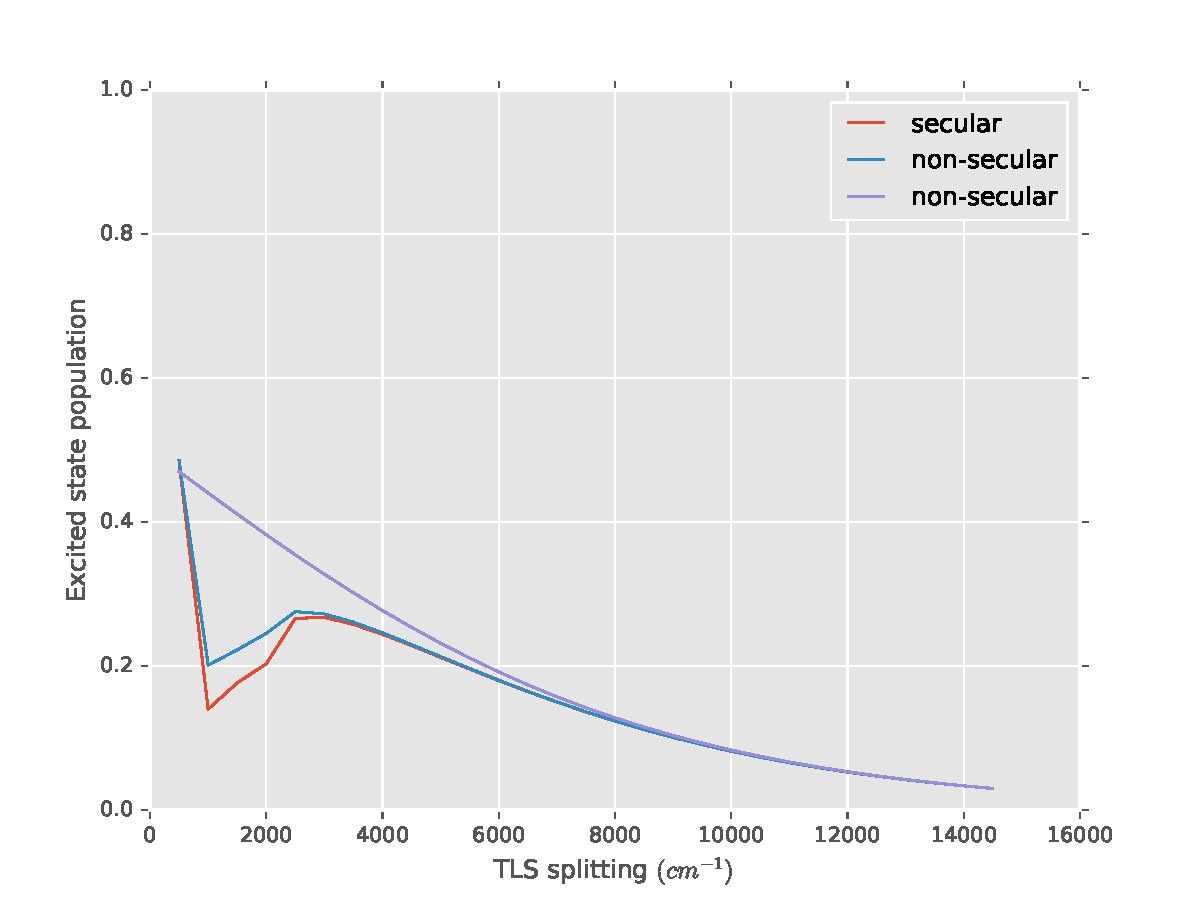
\includegraphics[width=0.8\textwidth]{Images/Checks/Pop_SS_divergence_a300_Tem6000_w0300_eps2000.pdf}
=======
	\includegraphics[width=0.8\textwidth]{"/home/henry/Work/phd-work/vibronic-TLS/Notes/Images/Checks/Pop_SS_divergence_a300_Tem6000_w0300_eps2000".pdf}
>>>>>>> .merge_file_pvGeVo
	\caption{Steady-state excited state population as a function of TLS splitting where $\alpha_{ph}=300$, $T_{EM} =6000$, $\omega_0 = 300$}
	\label{fig:steadyStatevsSplitting}
\end{figure}


\subsection{Underdamped Lorentzian Spectral Density (Localised vibrations)}
\begin{itemize}
	\item Large splitting, everything converges.
	\item As splitting decreases, the NS and S start to diverge from the naive. NS and S remain close until very small splitting, at which point the NS appears to return towards agreement with naive.
\end{itemize}

For moderate splitting and an underdamped phonon spectral density, the excited and ground states vibronic manifolds are well separated, see figures \ref{fig:manifold_weakcoupling}-\ref{fig:manifold_strongsmallsplitting}. This means that the dynamics are well approximated by the naive, electronic Lindblad theory of dissipation. However, if the electronic splitting becomes sufficiently small then the two manifolds can overlap and we start to observe the complex behaviour seen in the overdamped case. This happens at a much smaller splitting size since the ladder spacing of the vibronic states is so much smaller.

\begin{itemize}
	\item Is this occurring because the system is so far off resonance with the vibrations? (Reducing the splitting so it is closer to the peak of the spectral density indeed means vibronic theories diverge from the naive.)
\end{itemize}

\begin{figure}[h]
	\centering
<<<<<<< .merge_file_cKYZ1o
	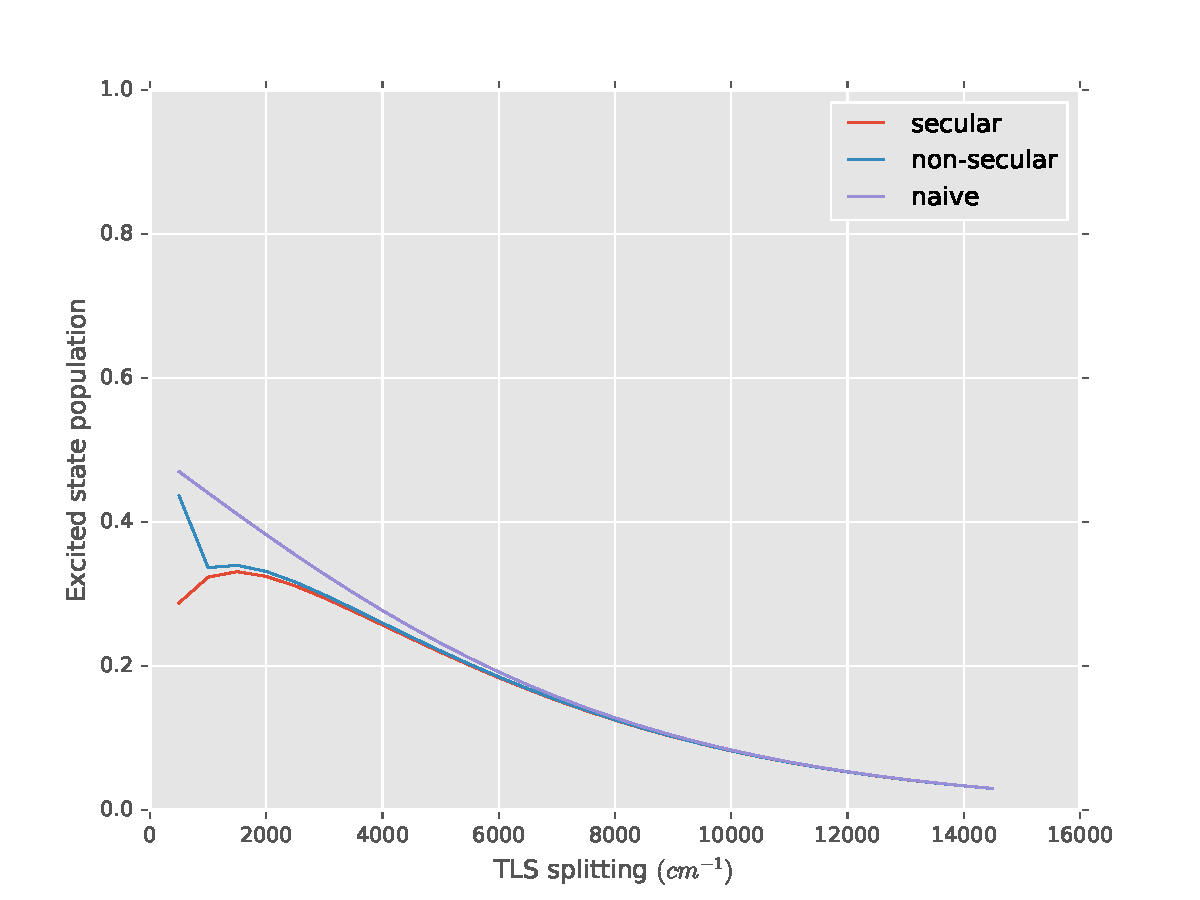
\includegraphics[width=0.8\textwidth]{Images/Checks/RealPop_SS_divergence_a300_Tem6000_w030_eps2000.pdf}
=======
	\includegraphics[width=0.8\textwidth]{"/home/henry/Work/phd-work/vibronic-TLS/Notes/Images/Checks/RealPop_SS_divergence_a300_Tem6000_w030_eps2000".pdf}
>>>>>>> .merge_file_pvGeVo
	\caption{Steady-state excited state population as a function of TLS splitting where $\alpha_{ph}=300$, $T_{EM} =6000$, $\omega_0 = 30$, $k_B T_{EM}=4170cm^{-1}$}
	\label{fig:steadyStatevsSplitting}
\end{figure}

\begin{figure}[h]
	\centering
	\begin{minipage}[b]{0.325\textwidth}
		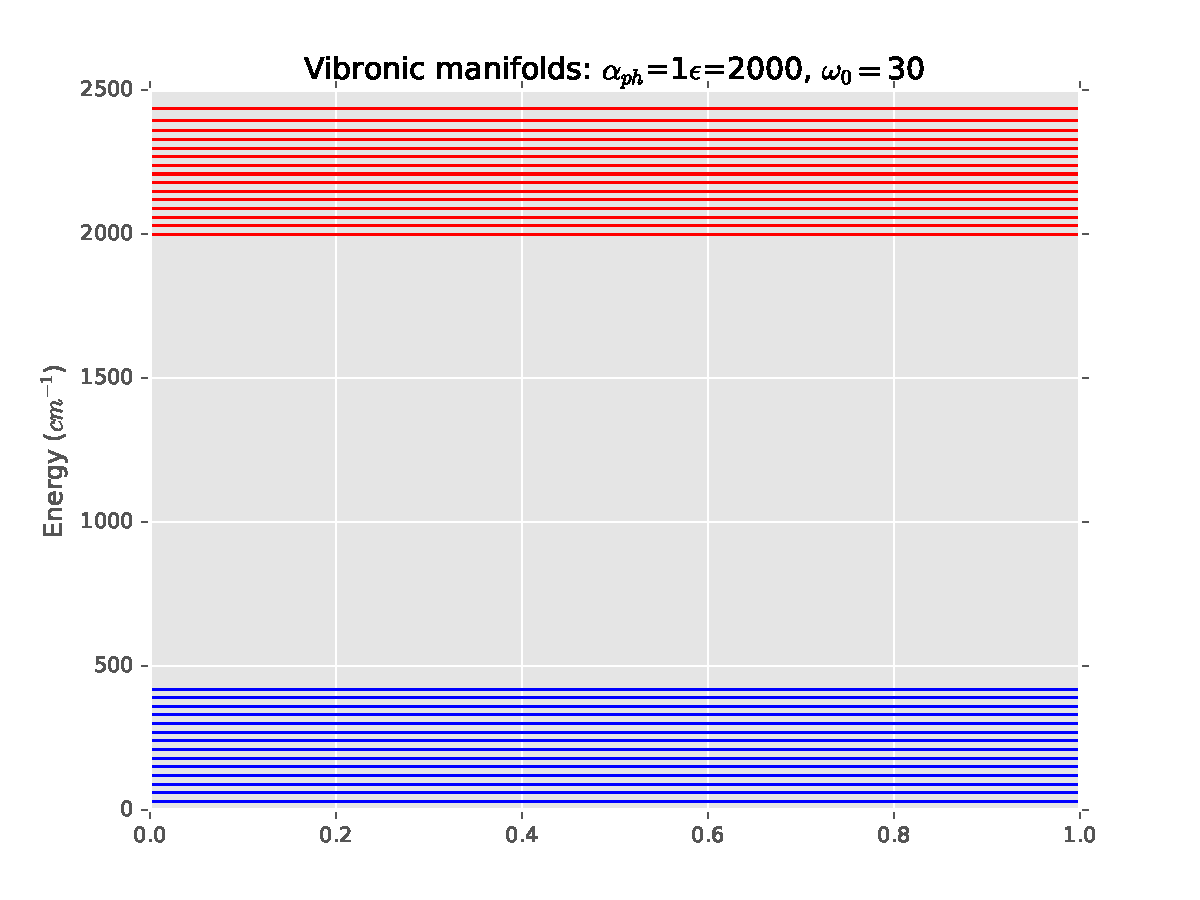
\includegraphics[width=\textwidth]{Images/Spectra/Manifolds_a1_Tph300_Tem6000_w030_eps2000.pdf}
		\caption{}
		\label{fig:manifold_weakcoupling}
	\end{minipage}
	\begin{minipage}[b]{0.325\textwidth}
		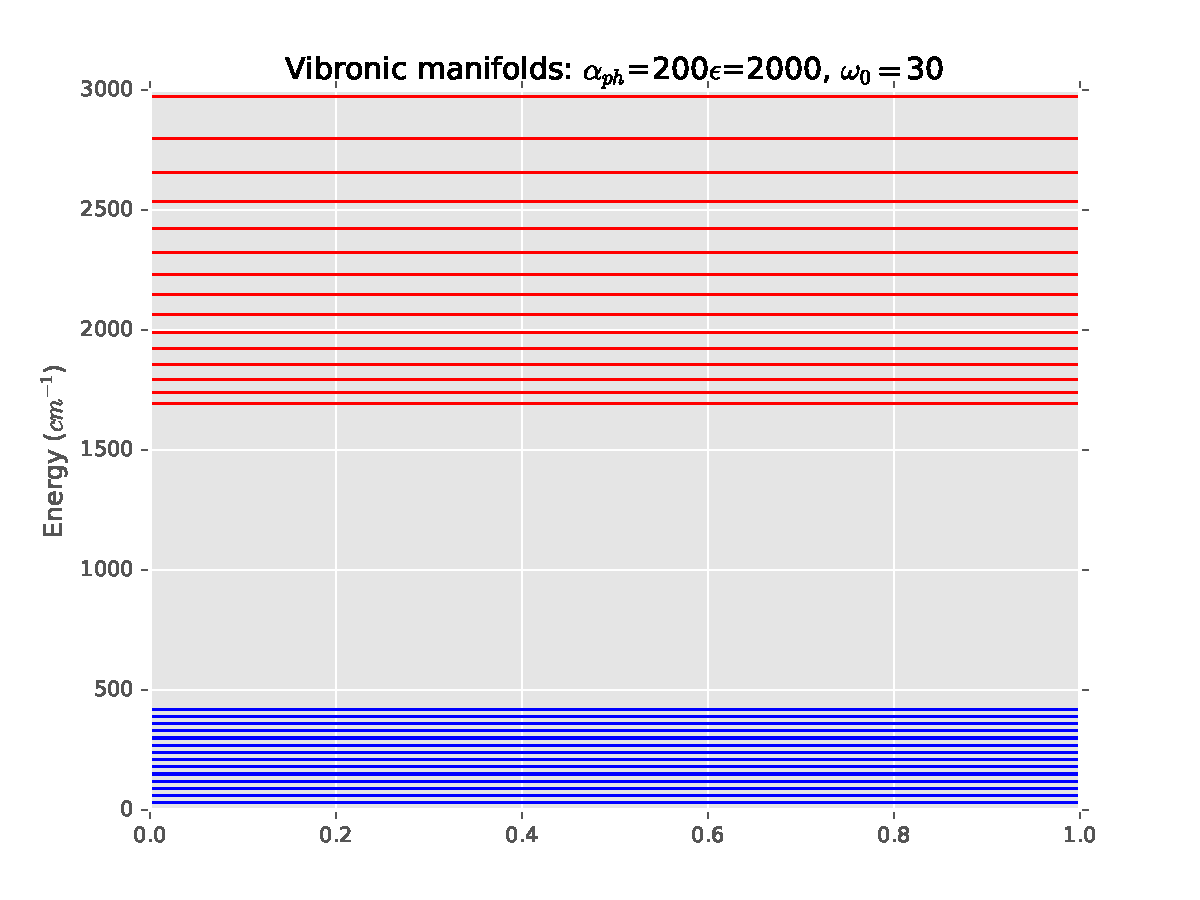
\includegraphics[width=\textwidth]{Images/Spectra/Manifolds_a200_Tph300_Tem6000_w030_eps2000.pdf}
		\caption{}
		\label{fig:manifold_stronglargesplitting}
	\end{minipage}
	\begin{minipage}[b]{0.325\textwidth}
		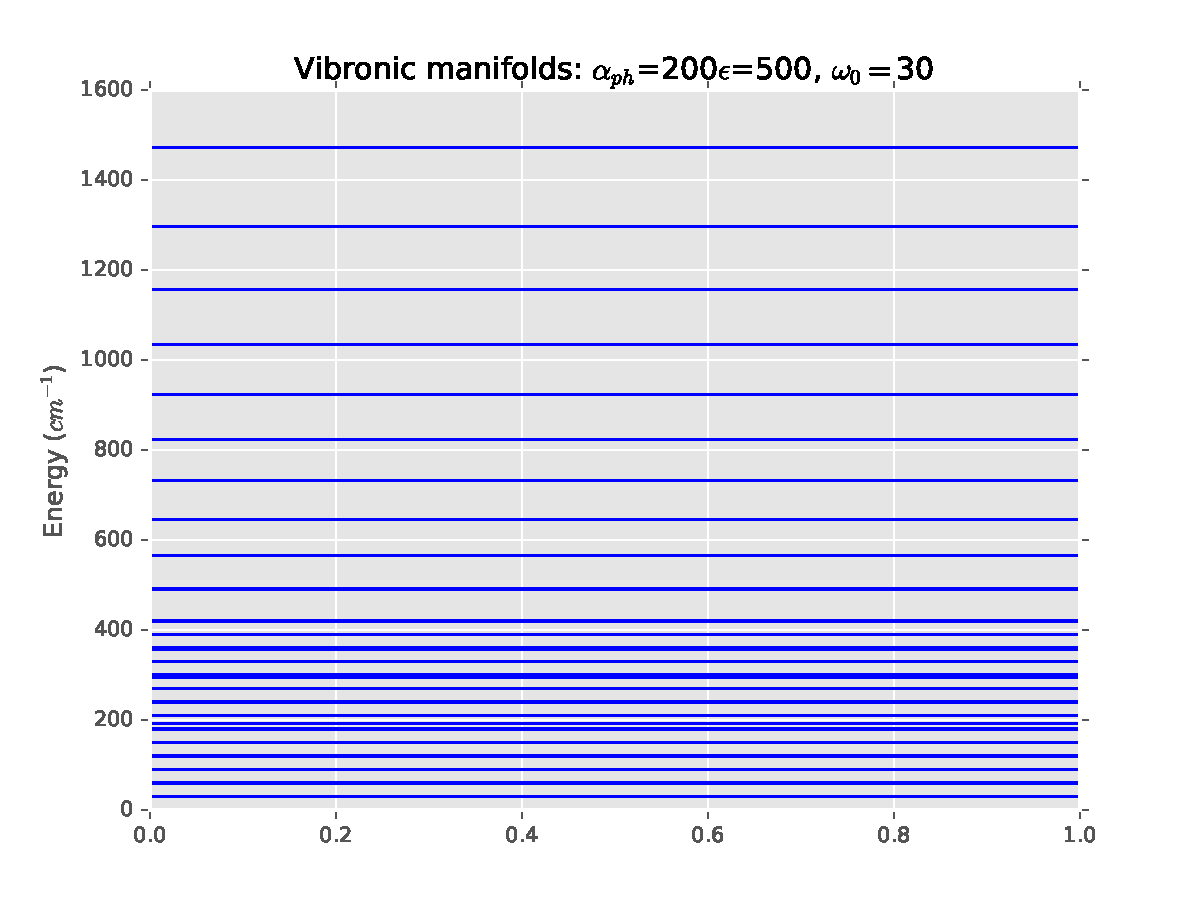
\includegraphics[width=\textwidth]{Images/Spectra/Manifolds_a200_Tph300_Tem6000_w030_eps500.pdf}
		\caption{}
		\label{fig:manifold_strongsmallsplitting}
	\end{minipage}
\caption{The vibronic manifold structure of the TLS with an underdamped Phonon spectral density. It can be seen that strong-coupling as well as small splitting can cause mixing of the vibronic levels.}
\end{figure}
\begin{comment}
\begin{figure}[h]
	\centering
<<<<<<< .merge_file_cKYZ1o
	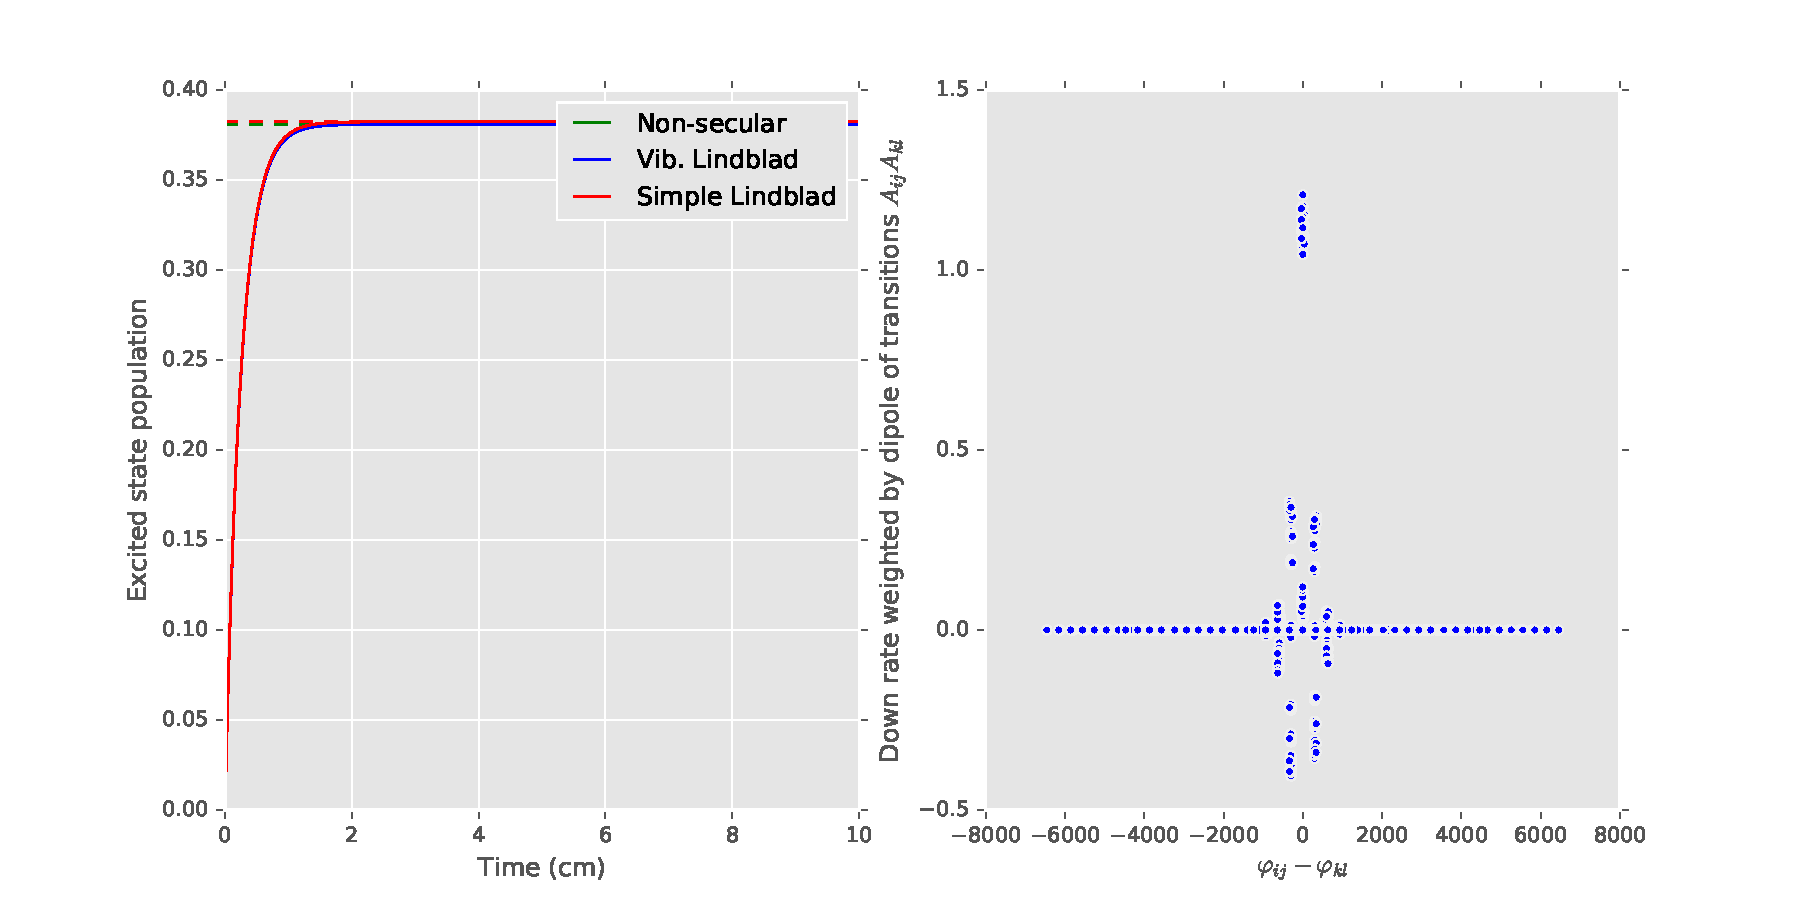
\includegraphics[width=\textwidth]{Images/Dynamics/Pop_a5_N15_Tem6000_w0300_eps2000.pdf}
=======
	\includegraphics[width=\textwidth]{"/home/henry/Work/phd-work/vibronic-TLS/Notes/Images/Dynamics/Pop_a5_N15_Tem6000_w0300_eps2000".pdf}
>>>>>>> .merge_file_pvGeVo
	\caption{Population where $\alpha_{ph}=5$, $T_{EM} =6000$, $\omega_0 = 300$, $\epsilon=10000$}
	\label{}
\end{figure}
\begin{figure}[h]
	\centering
<<<<<<< .merge_file_cKYZ1o
	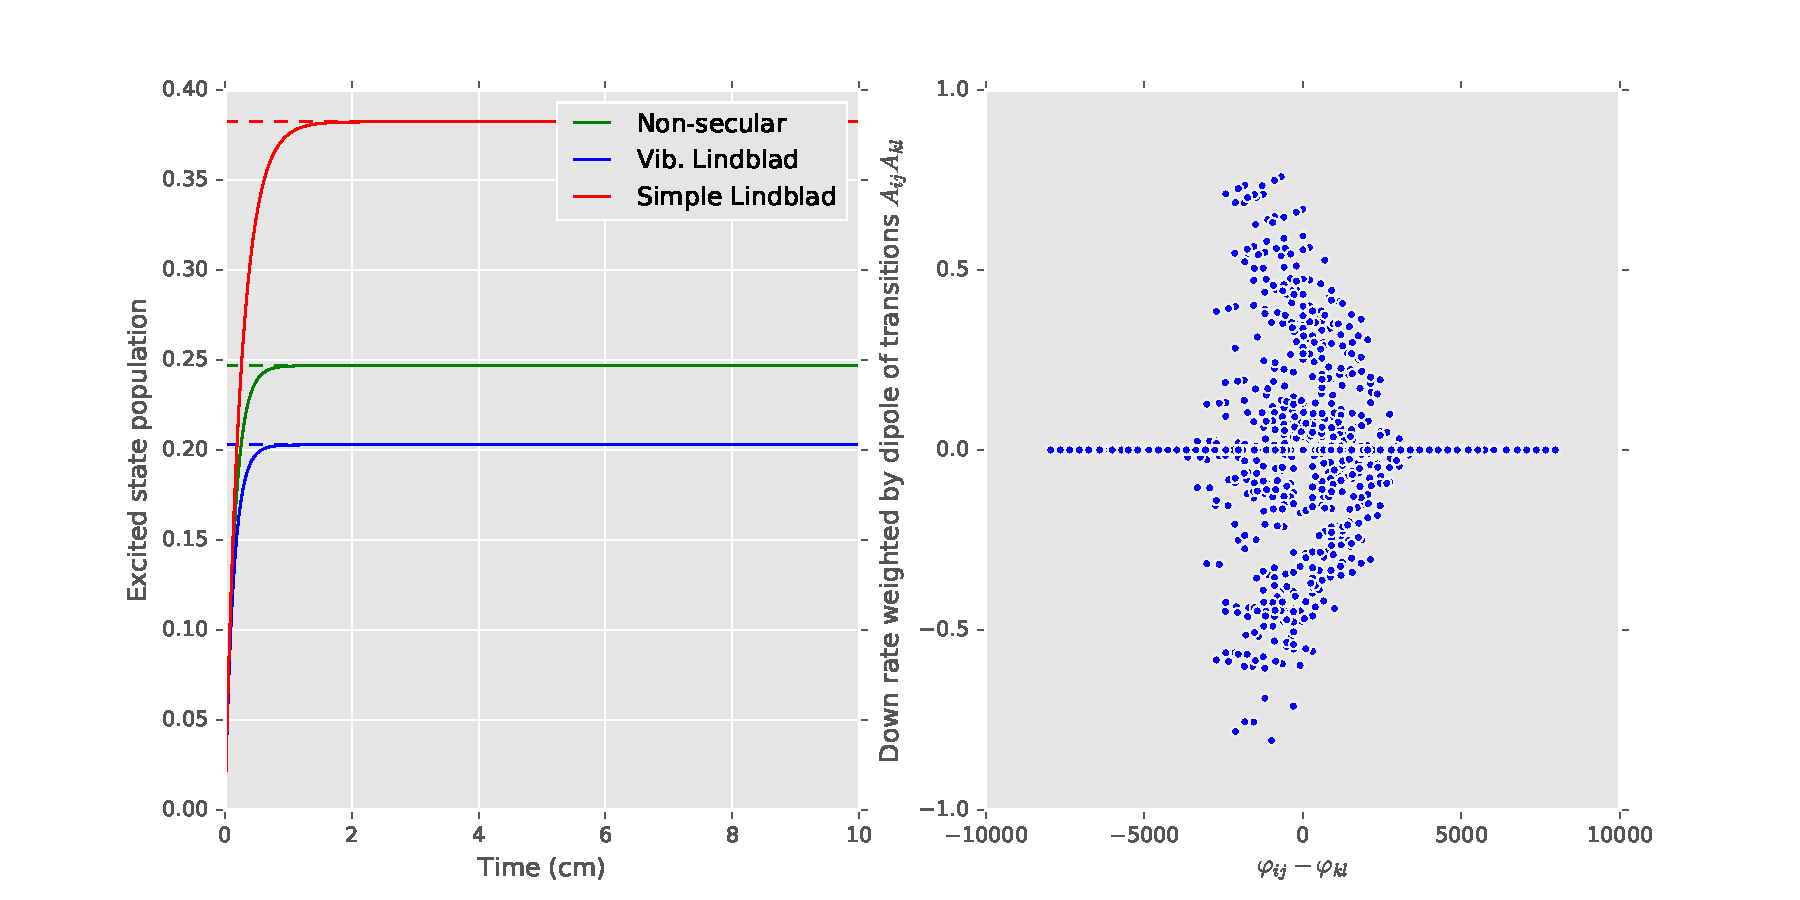
\includegraphics[width=\textwidth]{Images/Dynamics/Pop_a300_N15_Tem6000_w0300_eps2000.pdf}
=======
	\includegraphics[width=\textwidth]{"/home/henry/Work/phd-work/vibronic-TLS/Notes/Images/Dynamics/Pop_a300_N15_Tem6000_w0300_eps2000".pdf}
>>>>>>> .merge_file_pvGeVo
	\caption{Population where $\alpha_{ph}=300$, $T_{EM} =6000$, $\omega_0 = 300$, $\epsilon=2000$}
	\label{}
\end{figure}
\begin{figure}[h]
	\centering
<<<<<<< .merge_file_cKYZ1o
	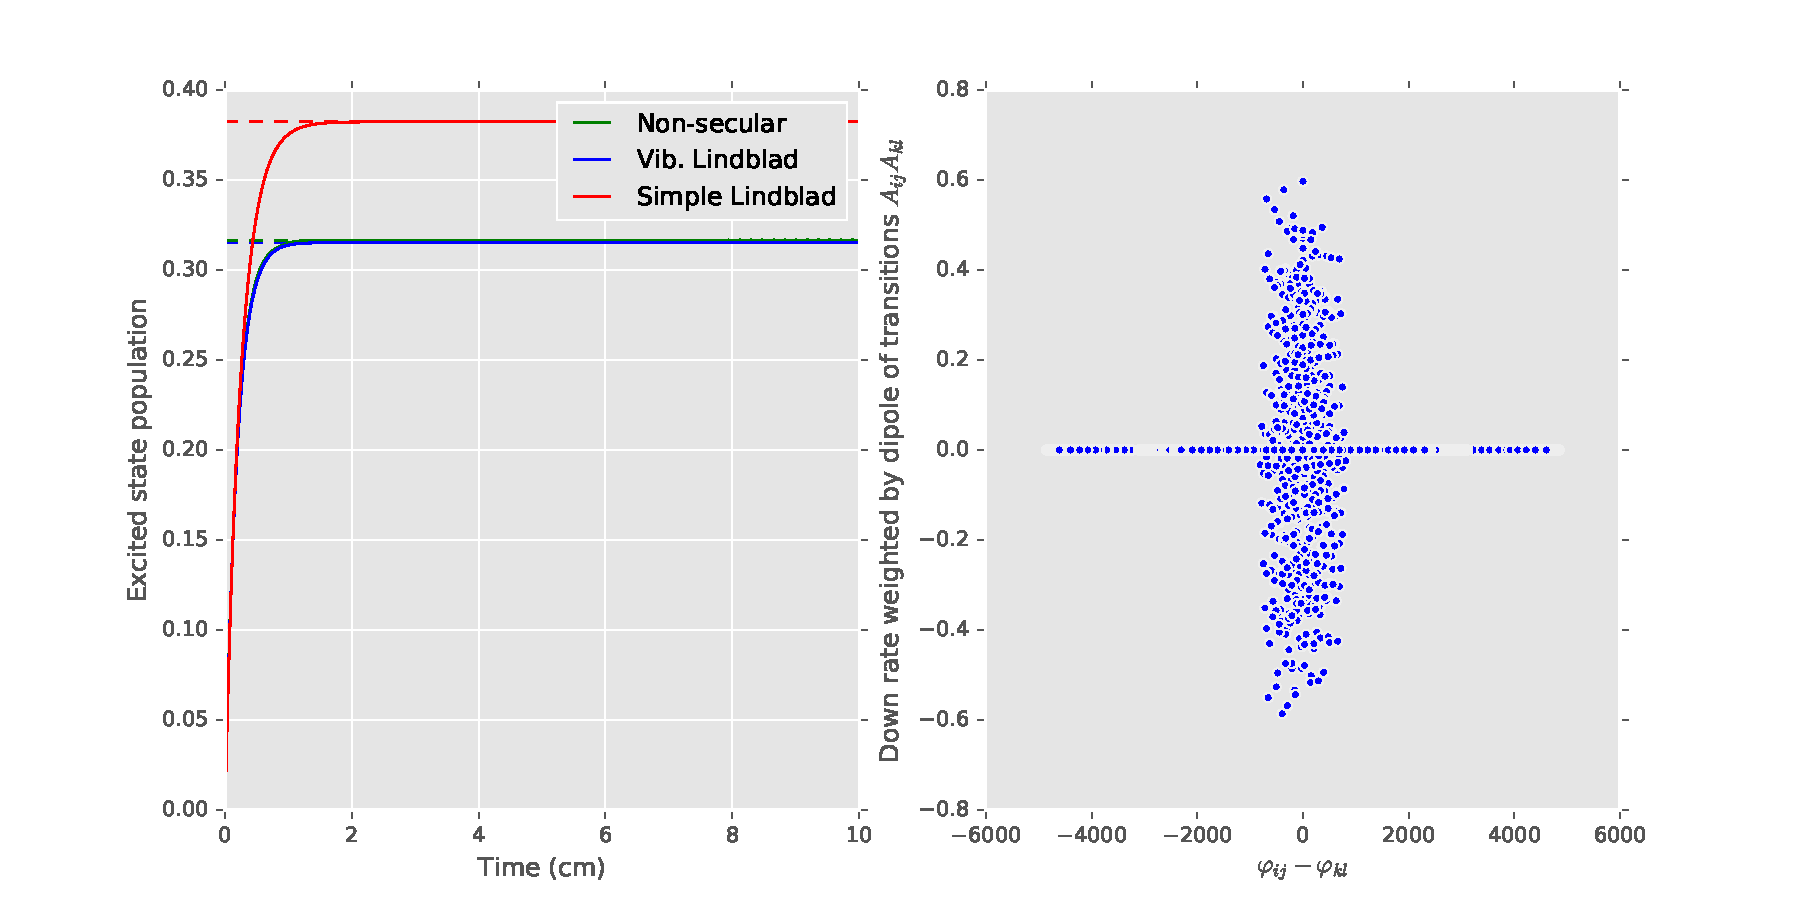
\includegraphics[width=\textwidth]{Images/Dynamics/Pop_a300_N15_Tem6000_w030_eps2000.pdf}
=======
	\includegraphics[width=\textwidth]{"/home/henry/Work/phd-work/vibronic-TLS/Notes/Images/Dynamics/Pop_a300_N15_Tem6000_w030_eps2000".pdf}
>>>>>>> .merge_file_pvGeVo
	\caption{Population where $\alpha_{ph}=300$, $T_{EM} =6000$, $\omega_0 = 30$, $\epsilon=2000$}
	\label{}
\end{figure}

\subsection{Validity of RWA}
\begin{itemize}
	\item Comparing \ref{ssec:nrwa} and \ref{ssec:nsec} find regimes where the two different Hamiltonians yield the same dynamics. Within these regimes, do they agree with the secular theories too? Therefore, does secular imply rotating-wave (at least in the dissipators)?
	\item It seems like the underdamped spectral density reduces the temperature dependence of the dynamics. For strong phonon coupling, non-secular is never equivalent to the secular theory.
\end{itemize}
\end{comment}
\section{Future work}

\subsection{Polaron shifts, phonon dynamics and optical spectra}

\begin{itemize}
	\item Does non-secularity alter the dynamics predicted by the Franck-Condon model for $T_{EM}=0$? No, at low temperature the theory is well approximated by the 
	\item As temperature increases, what happens to the equilibrium phonon positions?
	\item Think about polaron shifts. Does this cause the overlaps of excited and ground states to decrease? Does this lead to decrease in overlap between absorption and emission spectra?
	\item Do the calculations of Fluorescence spectra for electronic and non-secular theories in both the overdamped and underdamped phonon cases. See if the profiles match the theory that they are able to model localised and delocalised vibrations respectively.
\end{itemize}

<<<<<<< .merge_file_cKYZ1o

\bibliographystyle{ieeetr}
\bibliography{/Users/henrymaguire/Work/phd-work/BibTex/library}
=======
\subsection{Dimers and the nano-photocell}
\begin{itemize}
	\item In larger molecules there are going to be near degeneracies. Depending on a number of factors, this is going to result in charge transfer via vibronic resonances. Do we include this, or can we postulate that the important contributions are already included in the direct excitonic coupling? Need to think about the physics of this process.
\end{itemize}
\bibliographystyle{ieeetr}
\bibliography{/home/henry/Work/phd-work/BibTex/library}
>>>>>>> .merge_file_pvGeVo
\end{document}
